\Chapter{Étude de plasmas magnétisés}
\chaptermark{Étude de plasmas magnétisés}
\begin{refsection}
Ce quatrième chapitre porte sur l'étude de deux cas concrets,
chacun représentatif d'une configuration magnétique particulière : le filtre
magnétique avec le propulseur PEGASES et la colonne de plasma magnétisée de la
source d'ions négatifs CYBELE. 
A travers ces exemples, nous testons les possibilités du nouveau code MAGNIS,
tout en explorant la physique qu'il révèle. Les simulations sont discutées et
confrontées aux mesures expérimentales ainsi qu'aux résultats de modèles
statistiques.
En fin de chapitre, nous simulons une configuration typique de bord de tokamak,
de champ magnétique intense et où le transport est principalement de nature
turbulente. 
		 
\section{Barrière magnétique - PEGASES}
PEGASES, acronyme de \emph{Plasma Propulsion with Electronegative Gases}, est
un prototype de propulseur électrostatique à grille (PEG)
ion-ion\parencite{Chabert} conçu au LPP (Laboratoire de Physique des
Plasma) de l'École Polytechnique de Paris et qui a pour originalité d'éjecter à
la fois des ions négatifs et des ions positifs pour générer une poussée. Dans ce
nouveau concept prometteur, les faisceaux d'ions de charges opposées se
neutralisent mutuellement à la sortie du propulseur, rendant la cathode
neutralisante non nécessaire. Contrairement aux Propulseurs à Effet Hall
\footnote{Les propulseurs ioniques classiques, Propulseurs à Effet Hall (PEH),
sont constitués de trois étages : la source d'ion, l'étage d'accélération, où un
fort champ électromagnétique accélère les ions, et une cathode pour neutraliser
les ions positifs et éviter que le propulseur ne se charge.}, les PEG n'ont
pas de séparation entre les étages de création et d'accélération des ions.
Pour filtrer les électrons chauds et favoriser la création du plasma ion-ion, une
barrière magnétique d'une centaine de Gauss est placée entre la zone
d'ionisation et la région d'extraction.

\begin{figure}[htbp]
\centering
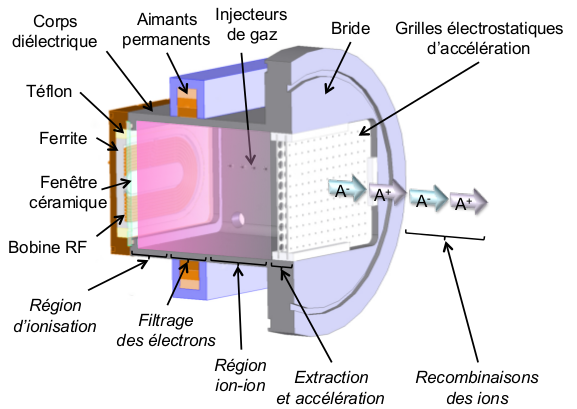
\includegraphics[width=0.75\textwidth]{figures/4-pegases3D.png}
{\caption{Schéma de principe de fonctionnement du propulseur PEGASES avec les
différents étages mentionnés en italiques\parencite{Popelier}.}
\label{4-pegases3D}}
\end{figure}

La structure en différents étages de PEGASES est représentée sur la
figure \ref{4-pegases3D}. Dans le premier étage, un gaz électronégatif est
excité inductivement par une puissance RF.
Le plasma de la source, constitué d'ion positifs, d'ions négatifs et d'électrons
est ensuite filtré par une barrière magnétique dans le deuxième étage du
propulseur. L'intensité de la barrière magnétique est choisie de façon à ce que
seuls les électrons soient magnétisés, laissant les ions diffuser librement à
travers le champ. Le plasma se sépare ainsi en deux régions de températures
électroniques différentes, l'une chaude du côté de l'injection de puissance,
l'autre plus froide en aval de la barrière, où se forme un plasma
ion-ion. Le troisième étage est enfin constitué du plasma ion-ion et
d'une série de grilles que l'on polarise pour extraire et accélérer les
particules, afin de former les faisceaux d'ions qui feront la poussée. La grille
d'extraction est la seule paroi conductrice du propulseur, ce qui permet de
contrôler le potentiel plasma en s'affranchissant du problème de l'état de
surface et de la contamination des parois\footnote{Dans les sources d'ion qui
utilisent des parois conductrices\ldots}.

La source ICP est entretenue à 4MHz avec une bobine plane dopée par un noyau de
ferrite protégée d'une fine (3mm) couche de céramique\parencite{Godyak} qui
peut fournir une puissance allant de 50W à 250W.
La géométrie de la source et la configuration du
filtre magnétique ont été choisies d'après les résultats de Aanesland \emph{et
al.}\parencite{Aanesland} qui donnent les conditions nécessaires à la
formation d'un plasma ion-ion. L'enceinte du propulseur, de dimension
12x12x8cm, est usiné à partir d'un bloc d'aluminium, anodisé afin de rendre
ses parois diélectriques. Une autre version, constituée de parois conductrices,
est aussi utilisée à des fins de diagnostique pour les éléments de la source.

Bien que MAGNIS ne puisse pas encore simuler les plasmas électronégatifs qui
nécessitent une description des interactions chimiques, il peut être utilisé
pour caractériser le transport complexe des électrons et du plasma en général à
travers le filtre magnétique. Pour étudier ce comportement, nous choisissons de
simuler un plasma d'argon, avec la géométrie présentée figure
\ref{4-pegasesSimDomain} :
\begin{figure}[htbp]
\centering
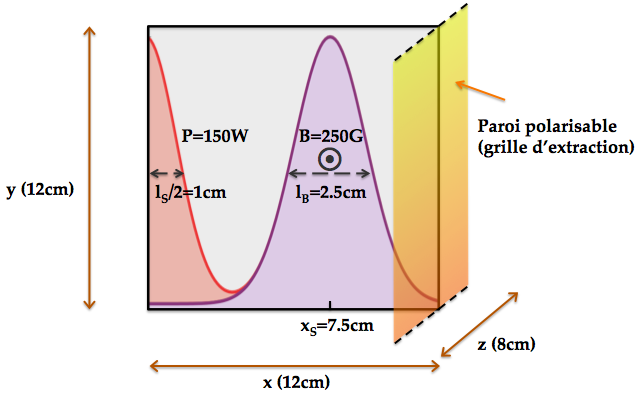
\includegraphics[width=0.6\textwidth]{figures/4-pegasesSimDomain.png}
{\caption{Le domaine de simulation est le plan perpendiculaire au champ
magnétique.}
\label{4-pegasesSimDomain}}
\end{figure}

Le domaine de simulation est rectangulaire et de
dimensions similaires à celles du prototype. La puissance est déposée dans la
région en amont du filtre magnétique sous la forme d'une demi-gaussienne de 2cm
de largeur. Le filtre magnétique est aussi de forme gaussienne, centré en
x=7.5cm et de largeur $\sim$ 2.5cm. Les parois seront choisies
conductrices ou diélectriques, avec une polarisation éventuelle de la grille
d'extraction (en jaune à droite du domaine). La puissance totale absorbée et la
densité de gaz sont fixées respectivement à 150W et 1mTorr.

Les types de solutions obtenues par MAGNIS dans le cas de parois diélectriques
et sans bias appliqué sont illustrées figure \ref{2-CartesWithTe} :

\begin{figure}[htbp]
    \centering
    \subfigure[]{\label{4-PegasesCarteDensiteBase}
    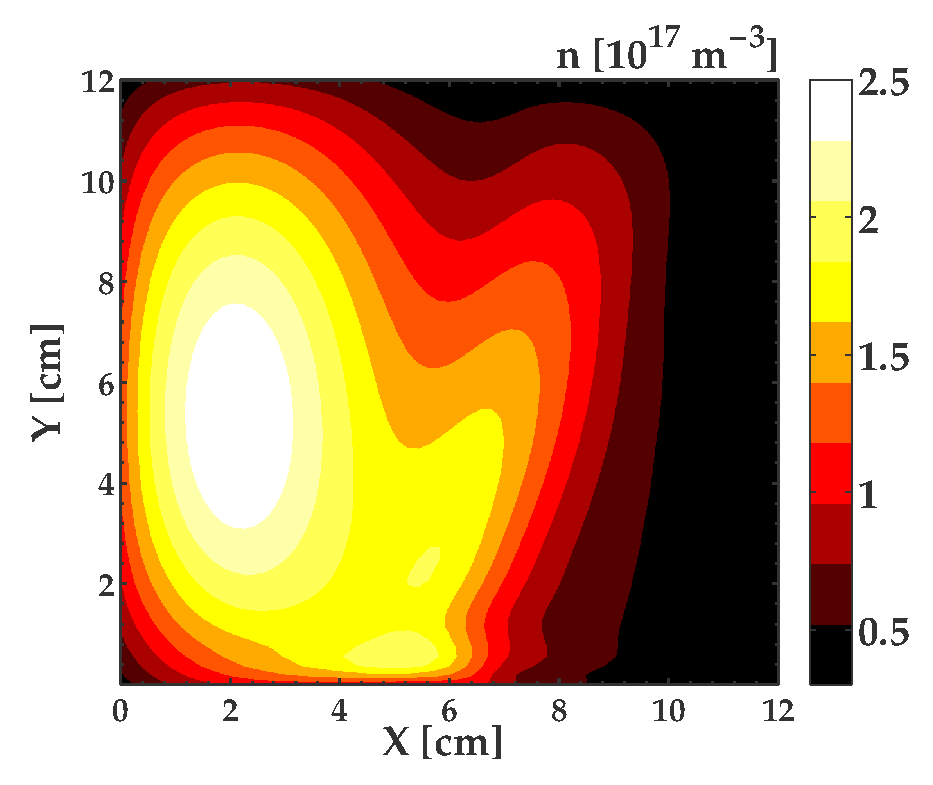
\includegraphics[height=5.75cm]{figures/4-PegasesCarteDensiteBase.eps}}
    \subfigure[]{\label{4-PegasesCartePotentielBase}
    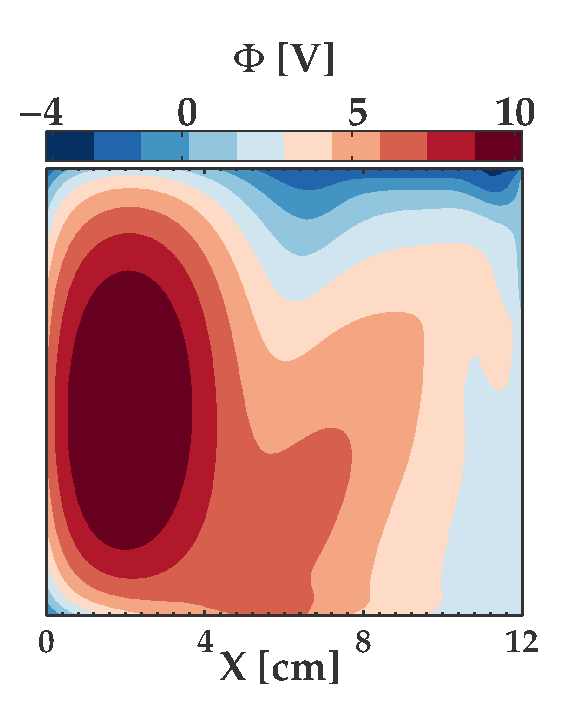
\includegraphics[height=5.75cm]{figures/4-PegasesCartePotentielBase.eps}}
    \subfigure[]{\label{4-PegasesCarteTemperatureBase}
    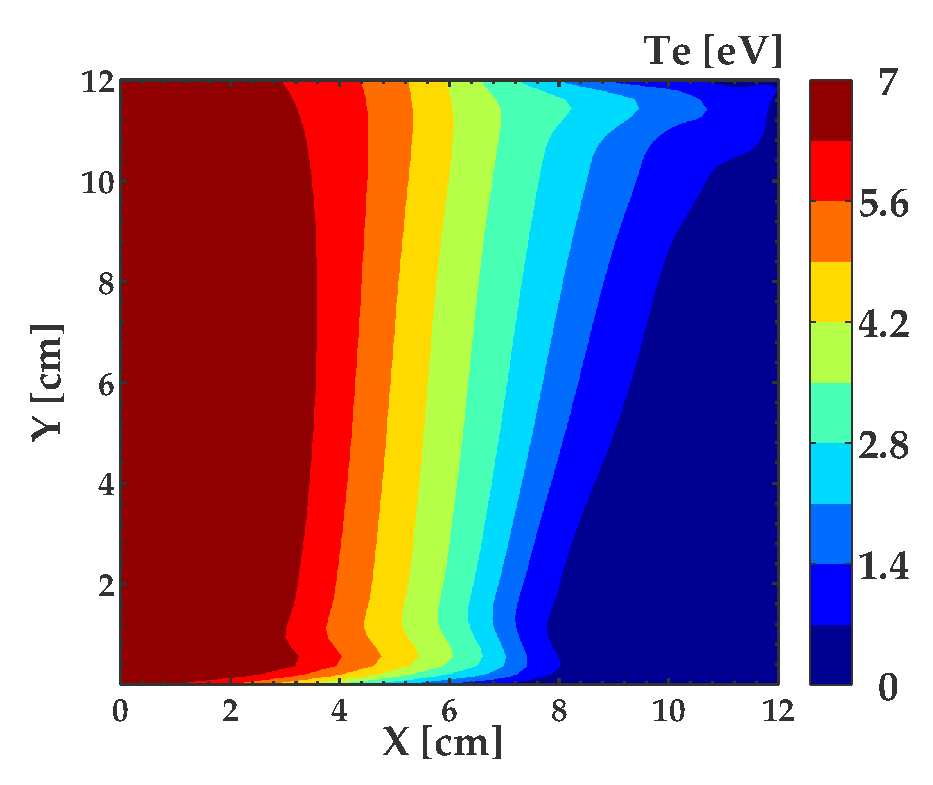
\includegraphics[height=5.75cm]{figures/4-PegasesCarteTemperatureBase.eps}}
    \caption{Cartes de densité \subref{4-PegasesCarteDensiteBase}~, de potentiel
    \subref{4-PegasesCartePotentielBase}~ et de température
    \subref{4-PegasesCarteTemperatureBase}~ dans le cas de parois
    diélectriques.}
    \label{2-CartesWithTe}
	\end{figure}

Le plasma atteint un état stationnaire en $\tau\simeq 10^{-4}\text{s}$. Le
maximum de densité de la source, 2.5x10$^{17}\text{m}^{-3}$ est atteint au
centre de la région d'ionisation. La densité du plasma décroît ensuite très
rapidement sur une longueur de 2 à 4cm. On peut observer de plus qu'une partie
du plasma diffuse en travers du champ magnétique. Le potentiel électrique, qui
suit le profil de densité, donne naissance à un champ électrique d'une centaine
de volt par mètre, quasiment ambipolaire dans la région non magnétisée, et
plutôt faible dans le filtre magnétique.

De manière conforme à la théorie, le filtre magnétique fait fortement décroître
la température électronique, la faisant chuter de 7eV à 1eV sur une
longueur de quelques centimètres. On peut aussi remarquer une légère asymétrie qui se met en
place le long de la direction Y. 

Dans ce type de configuration
magnétique les électrons, dont la mobilité est considérablement réduite,
cherchent un moyen de franchir le filtre afin de préserver la quasineutralité du
plasma. Les cartes de flux ioniques et électroniques présentées sur la figure~\ref{4-PegasesCarteFlux} permettent de se faire une idée de la dynamique
du système. Dans la zone non magnétisée, les ions issus de l'ionisation du gaz
sont créés avec une vitesse initiale quasiment nulle et tombent de façon
rectiligne aux parois. Du côté magnétisé, le flux augmente fortement puis est
ralenti à travers le filtre, mais celui-ci n'a pas d'influence notoire sur la
trajectoire des particules.

Le flux électronique est quant à lui bien moins évident à interpréter. La
caractéristique la plus immédiate à visualiser correspond au fort flux qui
remonte le long de la direction Y. Ce comportement se retrouve dans d'autres
sources utilisant un filtre magnétique, notamment dans la
sources d'ions négatifs de Garshing~\parencite{GarshingFiltre} et a été modélisé
dans ce contexte à travers différents
modèles, fluides et cinétiques\parencite{PIC2D-PIC3D-MAGMA}. On peut remarquer
deux autres phénomènes, moins détaillés dans la littérature : tout d'abord il
faut noter que le flux le plus important se situe dans la zone non magnétisée en
formant un vortex proche de la paroi à X=0cm qui reste à interpréter. Dans la
région en aval du filtre, on observe que le flux
électronique traverse le domaine en sens inverse, une partie
de celui-ci franchissant même à nouveau la barrière magnétique au niveau de la
paroi opposée.

\begin{figure}[htbp]
  \centering
    \subfigure[]{\label{4-PegasesCarteFluxIBase}
    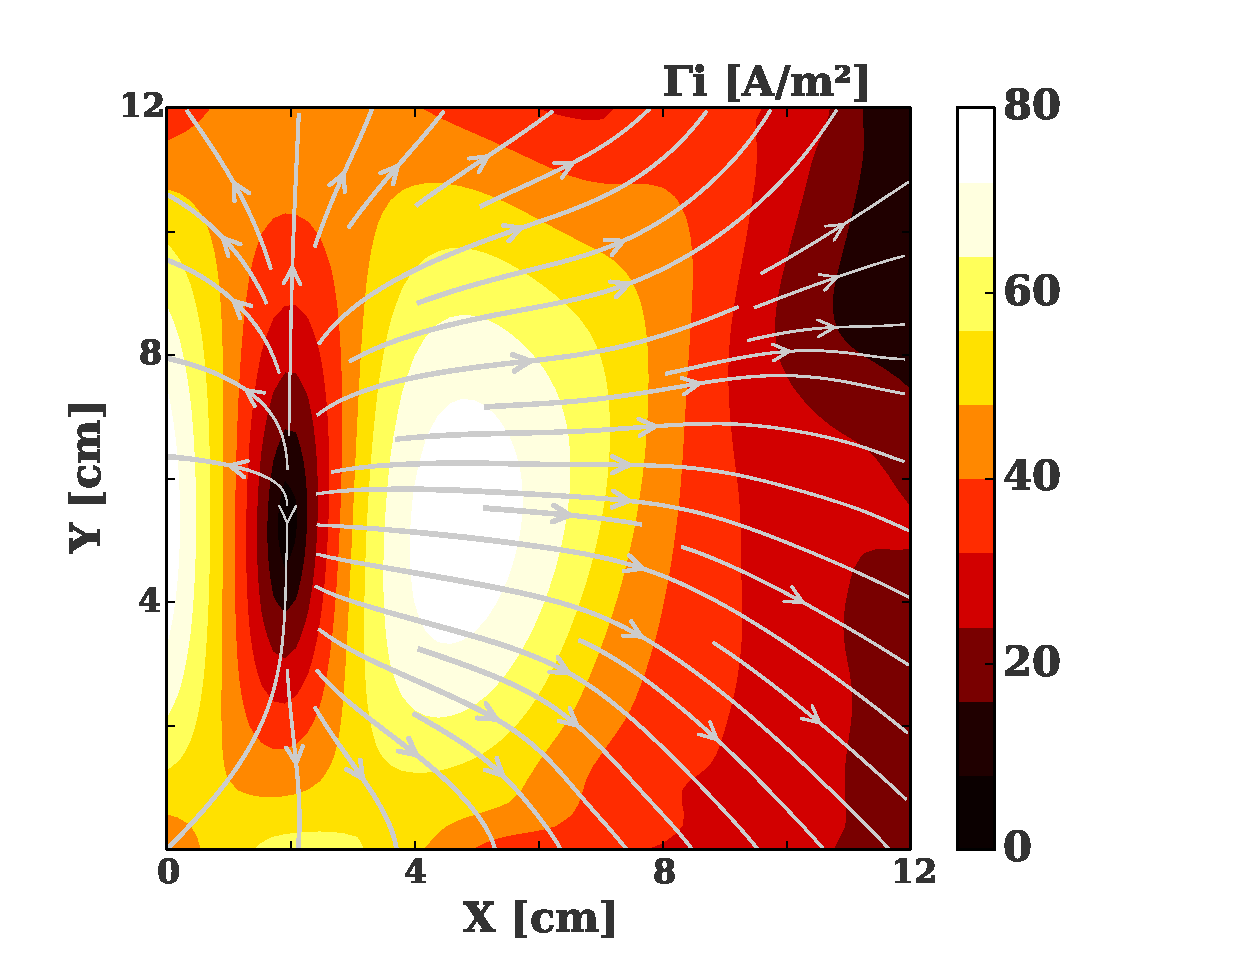
\includegraphics[height=6cm]{figures/4-PegasesCarteFluxIBase.eps}}
    \subfigure[]{\label{4-PegasesCarteFluxEBase}
    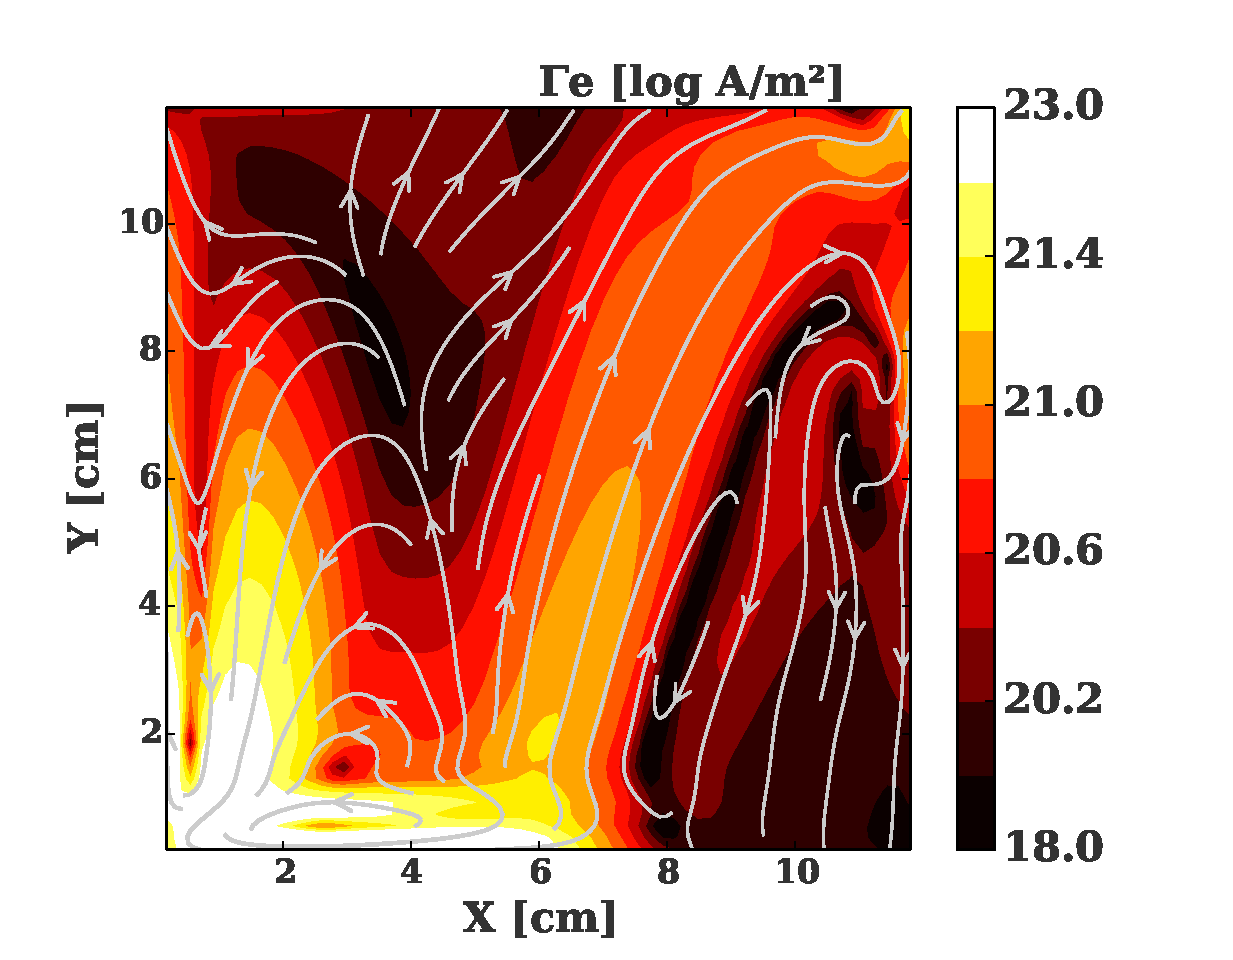
\includegraphics[height=6cm]{figures/4-PegasesCarteFluxEBase.eps}}
    \caption{Cartes de flux ionique \subref{4-PegasesCarteFluxEBase}~et de flux
    électronique \subref{4-PegasesCarteFluxEBase}~.}
    \label{4-PegasesCarteFlux}
\end{figure}

\subsection{Comparaison expérimentale}
Pour une première vérification du modèle, nous
comparons les résultats obtenus par Bredin sur l'étude de la
chute de température électronique en présence d'un champ magnétique
non-uniforme~\parencite{Bredin}. Nous reprenons et confrontons ainsi les mesures
effectuées à pression de gaz et champ magnétique variables. Dans ces expériences, la grille
d'extraction est enlevée, la source étant reliée à un grand volume diminuant
l'expansion spatiale du plasma. Pour nous placer au plus près des conditions
expérimentales, le domaine est allongé dans la direction X jusqu'à une longueur
de 24cm.
	
	\subsubsection{Scan en pression}
	Les comparaisons des profils de densité et de température présentées
	figure~\ref{pegasesCompPressProfils} sont en bon accords avec les mesures : à
	100mTorr, la densité du plasma atteint 10$^{18}\text{m}^{-3}$ puis décroît
	exponentiellement. La température électronique reste approximativement égale à
	2eV et n'est que faiblement impactée par le filtre magnétique. A 1mTorr, la
	densité diminue d'une décade et présente une sorte de palier dans la région de
	champ magnétique croissant que l'on devine dans les courbes expérimentales.
	
	La température, bien plus élevée à basse pression, part d'un maximum de 7eV à
	X=2cm et diminue à travers le filtre pour atteindre une valeur constante
	d'environ 1eV. On note cependant que le minimum de température n'est pas
	atteint exactement au même niveau que dans les expériences, celles-ci le
	plaçant au sommet de la barrière magnétique, et le modèle le
	prédisant plutôt à la fin du filtre, cette différence pouvant éventuellement
	être imputée à la géométrie du système dans le modèle.

\begin{figure}[htbp]
  \centering
    \subfigure[]{\label{4-pegasesCompPressDenProfile}
    
\includegraphics[height=5cm]{figures/4-pegasesCompPressDenProfile.eps}}
    \subfigure[]{\label{4-pegasesCompPressTempProfile}
    
\includegraphics[height=5cm]{figures/4-pegasesCompPressTempProfile.eps}}
    \caption{Profils de densité~\subref{4-pegasesCompPressTempProfile}~ et de
    température~\subref{4-pegasesCompPressTempProfile}~ pour trois pressions de
    gaz différentes, 1mtorr, 10mtorr et 100mtorr.}
    \label{pegasesCompPressProfils}
\end{figure}

	\subsubsection{Variations du champ magnétique}
	
	La comparaison des profils à différents champs magnétiques, présentée
	figure~\ref{4-pegasesCompMagProfile}, est un peu moins concordante. Les mesures
	expérimentales montrent en effet une augmentation de la densité et une
	température post-filtre de 2eV. Cependant, lors des mesures à 140G
	d'intensité de champ, on voit que le profil du filtre est aussi un peu plus
	large, pouvant éventuellement influencer les paramètres du plasma.
	
	\begin{figure}[htbp]
  \centering
    \subfigure[]{\label{4-pegasesCompMagDenProfile}
    
\includegraphics[height=5cm]{figures/4-pegasesCompMagDenProfile.eps}}
    \subfigure[]{\label{4-pegasesCompMagTempProfile}
    
\includegraphics[height=5cm]{figures/4-pegasesCompMagTempProfile.eps}}
    \caption{Profils de densité \subref{4-pegasesCompMagTempProfile}~ et de
    température \subref{4-pegasesCompMagTempProfile}~ pour trois intensité de
    champ magnétique 50G, 140G et 250G.}
    \label{4-pegasesCompMagProfile}
\end{figure}

Pour confirmer ces hypothèses, faisons varier la largeur de dépôt d'énergie
et la largeur de la barrière pour deux intensités de champ magnétique puis
comparons la densité maximale et la température des électrons après le
filtre~(voir le tableau \ref{4-pegasesCompLargeurs}). On voit ainsi que quand le
filtre est plus long, la densité augmente et la température baisse de façon plus
prononcée.
De l'autre côté, quand l'énergie est déposée sur une plus grande distance, la
densité a plutôt tendance à diminuer tandis qu'après la barrière, la
température électronique remonte.

\begin{table}
\footnotesize\centering
\ra{1.3}
\begin{tabular}{@{}ccccccc@{}}\toprule
\bfseries B&&\multicolumn{2}{c}{$l_B=2cm$} && \multicolumn{2}{c}{$l_B=4cm$}\\
\cmidrule{3-4} \cmidrule{6-7}
&& $n (m^{-3})$ & $\min T_e (eV)$ && $n (m^{-3})$ & $\min T_e (eV)$\\
\midrule 
250G\\
\scriptsize $l_S=2cm$ &&\bfseries\scriptsize 1.58
10\textsuperscript{17}&\bfseries\scriptsize 0.91&&\scriptsize 2.3
10\textsuperscript{17}&\scriptsize 0.73
\\
\scriptsize $l_S=4cm$  &&\scriptsize 1.4 10\textsuperscript{17} &\scriptsize
2.08&&\scriptsize 12 10\textsuperscript{17}&\scriptsize 1.38\\
140G\\
\scriptsize $l_S=2cm$ &&\scriptsize 1.57 10\textsuperscript{17} &\scriptsize
1.27&&\scriptsize 1.96 10\textsuperscript{17}&\scriptsize 0.98 \\
\scriptsize $l_S=4cm$  &&\scriptsize 1.39 10\textsuperscript{17} &\scriptsize
2.36&&\bfseries\scriptsize 1.75 10\textsuperscript{17}&\bfseries\scriptsize
1.6\\
\bottomrule
\end{tabular}
\caption{Tableau comparatif présentant la densité maximale du plasma ainsi que
la température électronique après le filtre magnétique pour des largeurs de
source d'énergie $l_S$ et de filtre magnétique $l_B$ différentes.}
\label{4-pegasesCompLargeurs}
\end{table}

Dans les mesures réalisées sur PEGASES, le filtre magnétique est respectivement
de largeur 4cm et 2cm dans les cas à 140G et 250G, ne laissant que deux
résultats "possibles" à prendre en considération. 
Les valeurs se rapprochant le plus des données expérimentales sont en gras dans
le tableau, elles correspondent à une largeur de source plus petite dans le cas fortement
magnétisé et inversement à une largeur de puissance déposée plus grande quand le
champ magnétique est plus étendu. L'influence de la taille de la zone de
chauffage n'est donc pas négligeable dans le cas des sources d'ion et semble de
plus varier en fonction de la configuration magnétique.

\subsection{Transport du courant dans le cas de parois conductrices}

La suite de cette étude porte sur le cas de parois
conductrices. Dans ce mode de fonctionnement, représentatif de l'une des
configurations de PEGASES ainsi que de nombreuses expérimentations,
l'application d'un bias positif sur la grille d'extraction afin d'extraire un
courant d'ions négatifs modifie aussi de manière conséquente les boucles de
courant, qui peuvent alors se refermer dans les parois (effet
Simon~\parencite{Simon54}).

Cet effet peut être particulièrement déterminant pour le transport global du
plasma dans le cas des parois qui interceptent les lignes de champ magnétique,
et où la gaine joue un rôle important dans l'évolution du potentiel jusqu'au
coeur de la source. A basse pression, les solutions deviennent instationnaires, et le transport
change radicalement de nature, devenant instable avec de violents phénomènes
intermittents.
	
\subsubsection{Influence du champ magnétique}
Dans les sources d'ions utilisant un filtre magnétique, c'est le courant
d'électrons qui est principalement responsable des inhomogénéités observées.
Théoriquement réduit d'un facteur en $1/B^2$ à travers le filtre dans une
analyse unidimensionnelle, on peut voir sur la
figure~\ref{pegasesVarMagCourantParoi} que le courant récupéré au niveau de la
grille d'extraction se comporte plutôt en $1/B$, ce qui est
généralement prit comme la signature de la présence d'un transport anormal.
Pourtant, dans ces sources, le transport reste classique et la raison de cette
augmentation significative doit être recherchée dans les effets de dérive
induits par le champ magnétique. Nous ne nous tenterons pas à
expliquer l'origine de transport, bien que la future utilisation de MAGNIS sera
possiblement d'une grande utilité pour aider à répondre à cette question.
Actuellement, même si les tentatives d'explications s'accordent sur la
traversée du filtre via la forte dérive ExB à proximité de la gaine, la
déviation du flux électronique en face du filtre reste incomprise.

\begin{figure}[htbp]
	\centering
	
\includegraphics[width=0.6\textwidth]{figures/4-pegasesVarMagCourantParoi.eps}
	{\caption{Courant total récupéré à la paroi en fonction de l'intensité du
	filtre magnétique pour trois voltages appliqués. }
	\label{pegasesVarMagCourantParoi}}
	\end{figure}

Attardons nous donc sur le flux électronique, à travers l'augmentation
progressive de l'intensité du champ magnétique. La
figure~\ref{4-pegasesfluxElectronique} représente une comparaison croisée du
flux d'électrons pour un champ magnétique variant de 0G à 500G et trois bias
différents de 0V, 10V et 20V appliqués à la source. 

Les trois premières cartes, en l'absence de filtre magnétique, montrent la
situation initiale pour les trois différents voltages. Cette situation, bien que
basique, est déjà intriguâtes, le flux électronique formant des
vortex en dehors de la région d'ionisation et remontant le long du
gradient de densité\footnote{Ce phénomène est hors de contexte du présent
manuscrit mais mérite tout de même d'être signalé, étant totalement absent de
la littérature.
Des simulations particulaires ont par ailleurs montré un comportement
similaire.}. On observe cependant que l'application du bias attire le flux
électronique qui peut alors atteindre dans le plasma une densité de courant de
quelques centaines d'ampère par mètre carré.

 \begin{figure}[htbp]
	\centering
	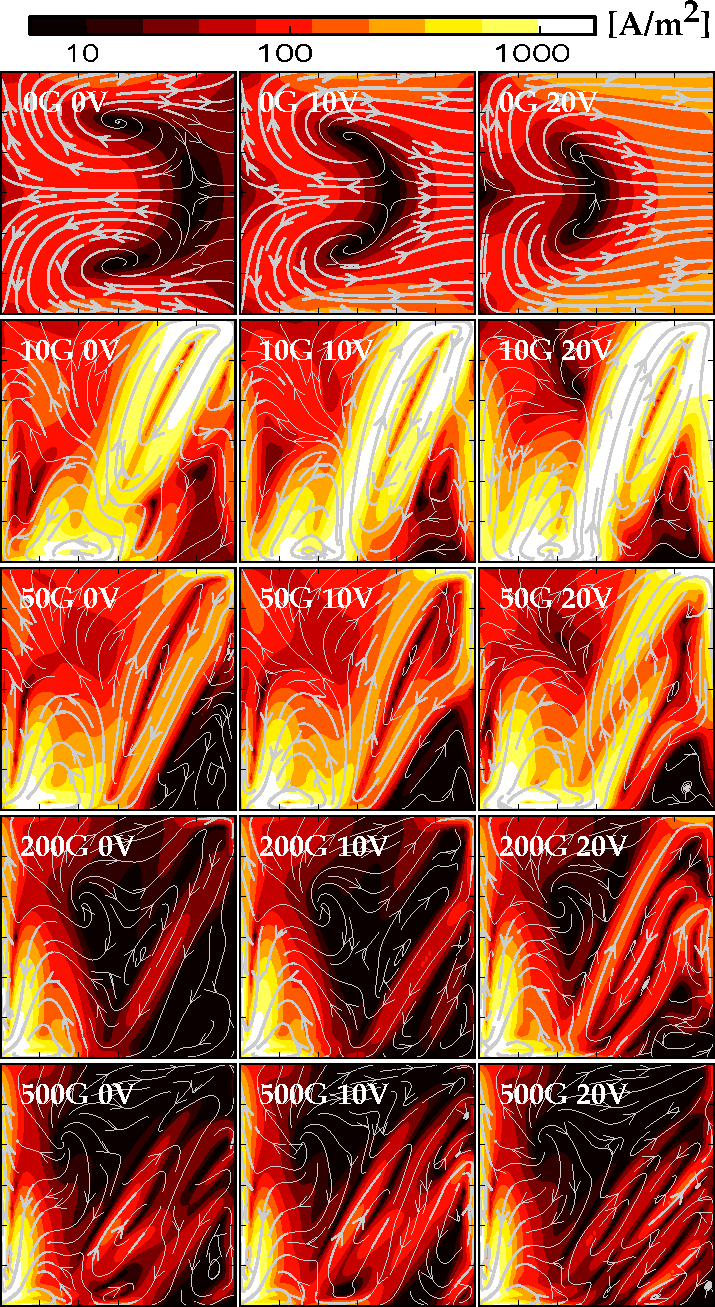
\includegraphics[width=0.85\textwidth]{figures/4-pegasesfluxElectronique.pdf}
	{\caption{Flux électronique à travers le filtre magnétique sur une plage
	allant de 0G à 500G pour trois différents voltages appliqués.}
	\label{4-pegasesfluxElectronique}}
	\end{figure}
	
L'apparition du filtre magnétique, à faible intensité de champ, modifie
complètement le flux électronique : la densité de courant devient asymétrique et
décuple d'intensité dans le bas de la région d'ionisation. A 10G, la
température électronique est de l'ordre de 5eV, donnant un rayon de Larmor
électronique d'environ 5mm. Les électrons sont déjà magnétisés et ne peuvent
traverser le filtre qu'au niveau de la paroi située en Y=12cm. Le flux
d'électrons se sépare ensuite pour rejoindre les ions qui ont traversé la
barrière sans perturbation, une partie plus ou moins importante allant à la
paroi en fonction du bias et l'autre traversant le domaine en sens inverse
jusqu'à atteindre la paroi en Y=0cm.

A 50G, l'intensité du courant électronique reste importante et un phénomène de
rotation des électrons autour de la barrière magnétique devient plus clair.
L'application du bias montre aussi que le flux pénètre sur quelques centimètre
dans la partie basse du filtre. A 200G et sans bias appliqué, le flux
électronique est fortement réduit à travers la barrière et change encore de
forme : le premier courant qui remontait le long du champ magnétique devient
moins important que le flux de retour. L'application d'un bias ou l'augmentation
de l'intensité de la barrière mène alors à l'apparition d'un phénomène instable
que nous allons regarder plus en détail dans la partie suivante.

\subsection{Phénomènes intermittents, instabilités}
A faible champ magnétique ou à pression suffisamment élevée, les solutions
obtenues par MAGNIS sont stationnaires, validant à posteriori l'hypothèse
d'approximation de l'inertie qui fonde les modèles de dérive-diffusion.
Cependant, lorsque la pression diminue, le transport collisionnel n'est plus
dominant et des phénomènes instables, caractéristiques des plasmas
magnétisés, peuvent apparaître et affecter toute la dynamique du système. 
 
	\subsubsection{Vagues ioniques}
La première instabilité que l'on voit apparaître est illustrée
figure~\ref{4-PegasesCarteDensiteWaves}. A intervalles régulières, un front
de surdensité traverse le filtre magnétique à très grande vitesse. La direction
 de propagation est perpendiculaire au front de densité, à l'oblique entre le
 champ magnétique et son gradient. Sans bias et à une pression de gaz de 1mTorr,
 les fronts de densité apparaissent à une fréquence d'environ 120kHz et se
 déplacent à une vitesse approximative de 2.2 km.s$\puissance{-1}$. 
 
\begin{figure}[htbp] 
  \centering
    \subfigure[]{\label{4-PegasesCarteDensiteWaves}
    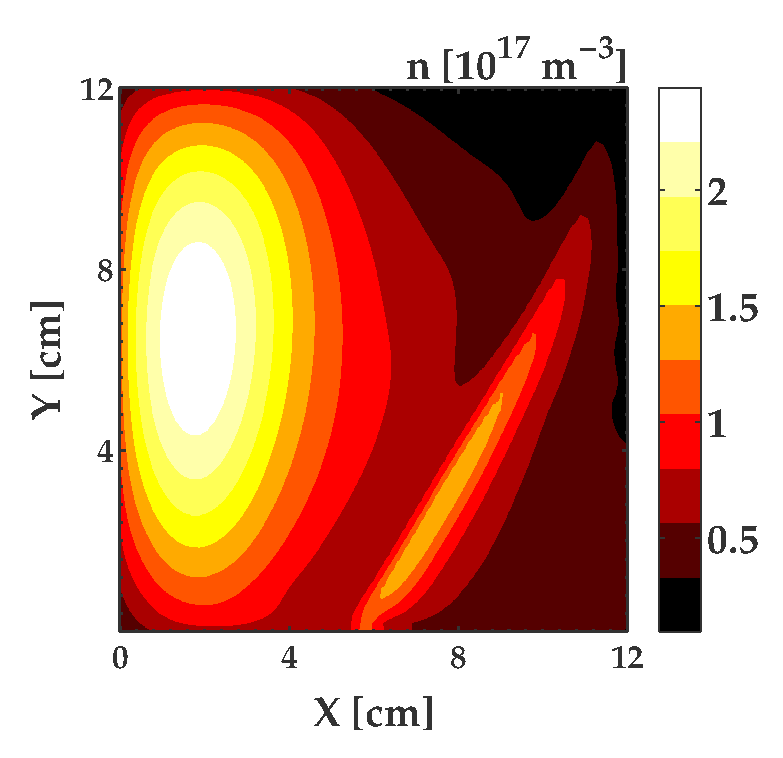
\includegraphics[height=5cm]{figures/4-PegasesCarteDensiteWave.eps}}
    \subfigure[]{\label{4-PegasesCarteViSurTeVarBias}
    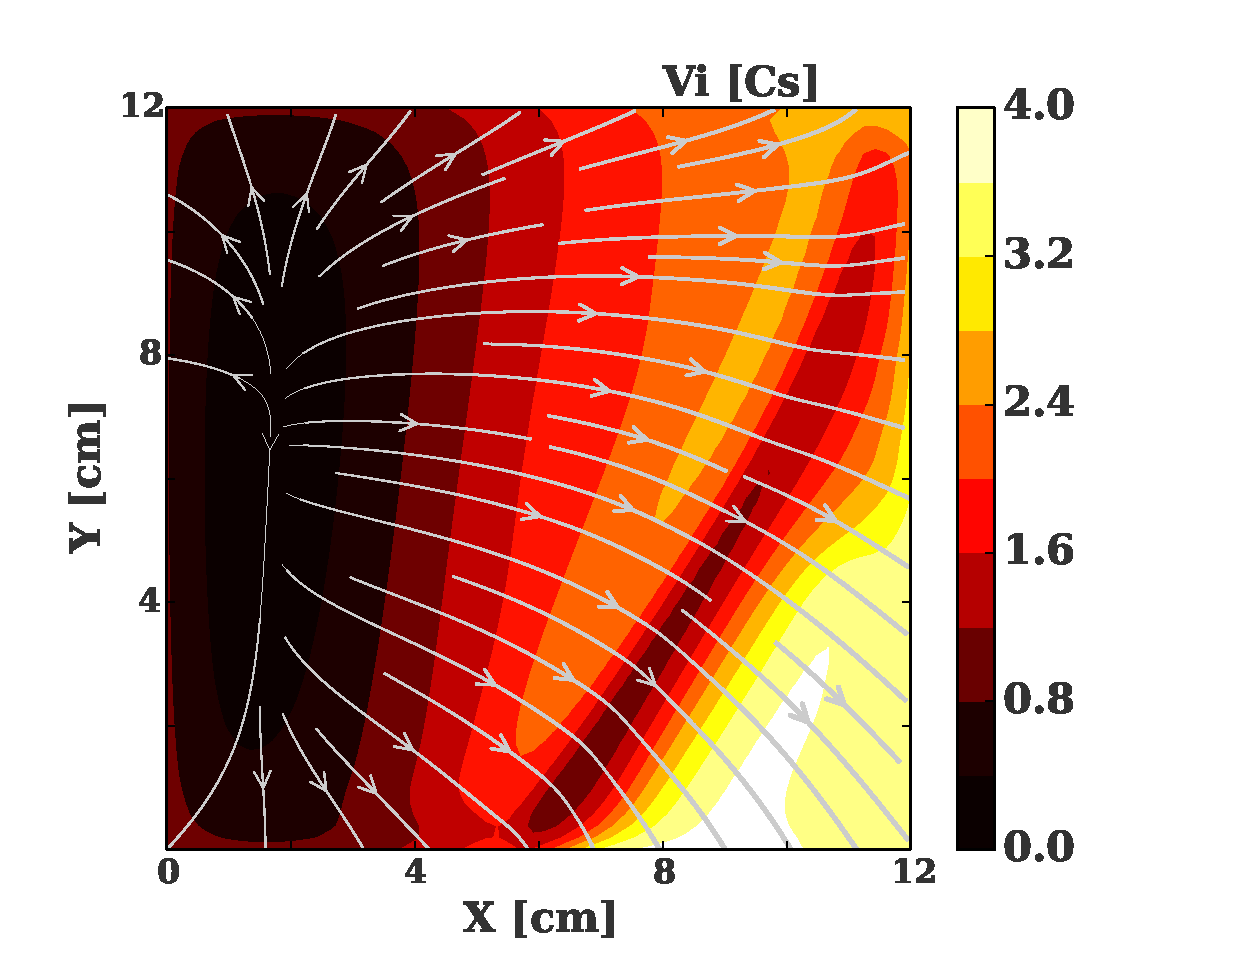
\includegraphics[height=5cm]{figures/4-PegasesCarteViSurTeVarBias.eps}}
    \caption{Cartes de densité~\subref{4-PegasesCarteDensiteWaves}~ et de
    nombre de Mach~\subref{4-PegasesCarteViSurTeVarBias} pour un champ
    magnétique de 250G, une densité de neutre de 1mTorr et un bias appliqué de
    20V.}
    \label{4-PegasesVaguesIoniques}
\end{figure}
 
 La figure~\ref{4-PegasesCarteViSurTeVarBias} représente la vitesse ionique
 rapportée à la vitesse de Bohm, ie. le nombre de Mach de
 l'écoulement ionique. On voit tout d'abord qu'une grande partie du domaine est
 occupée par des ions dont la vitesse dépasse la vitesse acoustique locale. En
 effet, les ions franchissent Mach1 le long du gradient de température, à
 $T_e\sim 5eV$ puis accélèrent encore jusqu'à atteindre Mach2 avant le front de
 densité. La vitesse décroît ensuite lors de la traversée de la surdensité, tout
 en restant supérieure à la vitesse de Bohm. La vitesse calculée du
 front est cependant inférieure à la vitesse des particules le constituant,
 soulignant le caractère ondulatoire de cette surdensité. Ce phénomène fait
 naturellement penser à la transition subsonique-supersonique qui advient dans
 les gaz compressibles classiques, où le front de densité serait l'onde
 acoustique résultante du passage des ions supersoniques. La vitesse de
 propagation de l'onde permet ainsi de définir une température critique :
 
 \begin{equation}
 	V_f=C_{s}=\sqrt{\frac{eT_e}{Zm_i}}\simeq 2.2\;10^{3}\,\text{m.s}^{-1}
 	\Leftrightarrow T_e\simeq 2\,\text{eV}
 \end{equation}
 
 Quelques propriétés peuvent être immédiatement dégagées. L'apparition et
 certaines particularités de cette instabilité sont directement reliées au
 gradient de température électronique et au terme d'inertie  :
 
 \begin{itemize}
   	\item Les solutions du modèle quand le terme inertiel d'advection est
	négligé sont stationnaires.
   \item Un plasma isotherme s'étend dans le sens du flux d'électron
   transverse et atteint lui aussi une solution stationnaire.
   \item la direction des fronts d'ondes est fortement corrélée au gradient
   de température.
\end{itemize}

La réponse à la polarisation de la grille d'extraction est aussi une autre
caractéristique intéressante de ce phénomène. Les
figures~\ref{4-PegasesCarteDensiteVarBiasWave}~
\subref{4-PegasesCarteDensiteVarBias1}~ \subref{4-PegasesCarteDensiteVarBias2}~
et~\subref{4-PegasesCarteDensiteVarBias3}~ illustrent cet effet en partie : la
dynamique des fronts, de vitesse approximativement constante à 0V, se décompose
en deux temps après l'application d'un faible voltage. Les fronts ralentissent
au niveau du maximum du filtre magnétique, augmentent en densité, puis sont
propulsés vers les parois après un certain temps de latence. A 30V, le champ
électrique freine si bien les ions qu'un bras de densité équivalente à celle du
plasma de la region d'ionisation se forme. 
	
	\begin{figure}[htbp]
  \centering
    \subfigure[]{\label{4-PegasesCarteDensiteVarBias1}
    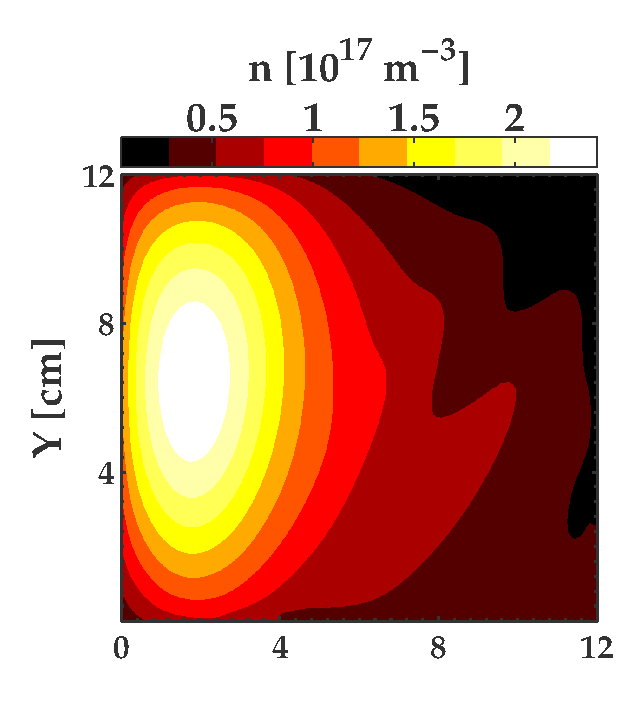
\includegraphics[height=6cm]{figures/4-PegasesCarteDensiteVarBias1.eps}}
    \subfigure[]{\label{4-PegasesCarteDensiteVarBias2}
    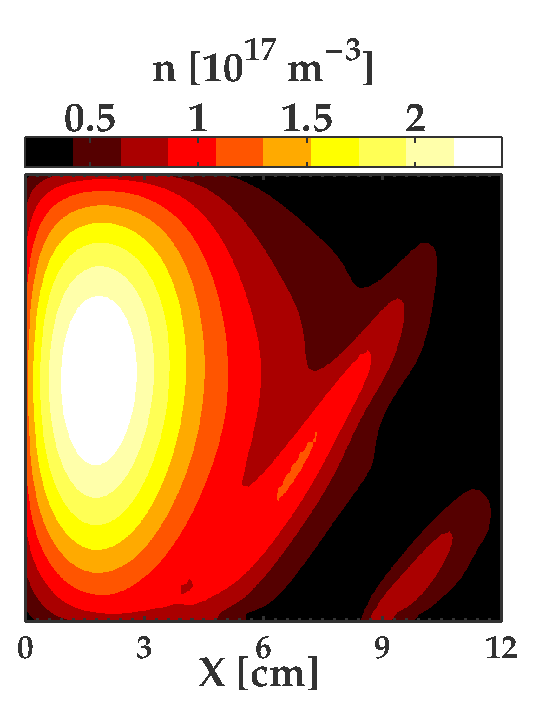
\includegraphics[height=6cm]{figures/4-PegasesCarteDensiteVarBias2.eps}}
    \subfigure[]{\label{4-PegasesCarteDensiteVarBias3}
    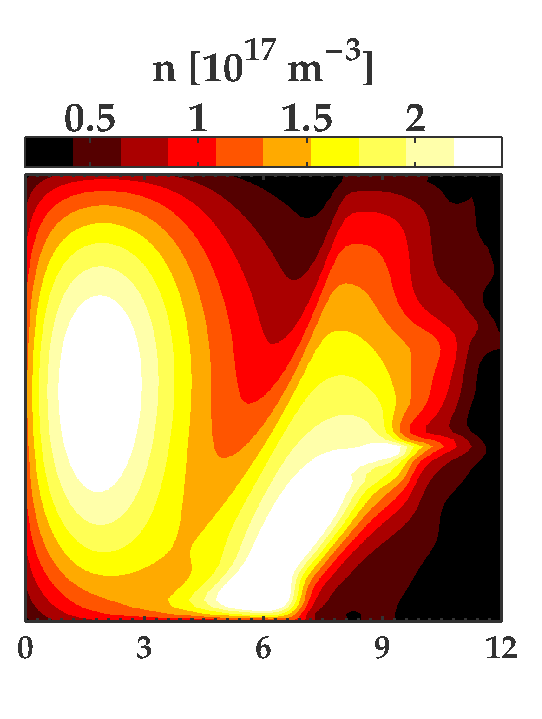
\includegraphics[height=6cm]{figures/4-PegasesCarteDensiteVarBias3.eps}}
    \caption{Cartes de densité\subref{4-PegasesCarteDensiteVarBias1}~, de
    potentiel\subref{4-PegasesCarteDensiteVarBias2}~ et de
    température\subref{4-PegasesCarteDensiteVarBias3}}
    \label{4-PegasesCarteDensiteVarBiasWave}
\end{figure}

On peut maintenant raccorder l'étrange flux électronique qui apparaissait dans
les cas fortements magnétisés de la
figure~\ref{4-PegasesCarteDensiteVarBiasWave}. Un champ éléctrique se forme
entre les fronts de densité, et se combine au filtre
magnétique pour faire naître un mouvement de dérive du type ExB, exacerbant le
transport des électrons au travers de la barrière. 

Enfin, il faut toutefois relever que le modèle n'arrive pas à atteindre 
une fréquence ou une longueur d'onde caractéristique pour ces oscillations,
celles-ci n'ayant pas convergées lors des tests sur maillage\footnote{La
vitesse des particules ainsi que celle des fronts d'onde semblent quant-t-à
elles indépendantes du maillage.}.
La caractérisation complète de cette instabilité est donc pour le moment
assez difficile à réaliser.
Pour terminer, on peut se poser la question de la réalité physique de
ce phénomène, qui n'a apparement pas été remarqué lors des expérimentations. La
présence d'ions supersoniques ne serait pourtant pas surprenante, étant donné
les gradients extrêmes, la très faible température électronique 
après le filtre, et la forte tension retenant le flux ionique.
Des simulations PIC récemment lancées au GREPHE sur une géométrie similaire
semblent montrer un comportement similaire, ce qui nous conforte dans les
résultats du modèle.

	\subsubsection{Instabilité liée au gradient de densité}
	A plus haute pression (10 mTorr et 100 mTorr), la variation de la tension
	appliquée à la grille d'extraction révèle une autre instabilité qui prend la
	forme de vaguelettes le long des gradients de densité (cf.
	figure~\ref{4-PegasesCarteDensiteVarBias5}). On peut aussi la voir apparaître
	le long des fronts de densité, au niveau des parois, dans des
	simulations isothermes ou encore dans le cas de la colonne de plasma. 
	
	\begin{figure}[htbp]
  \centering
    \label{4-PegasesCarteDensiteVarBias5}
    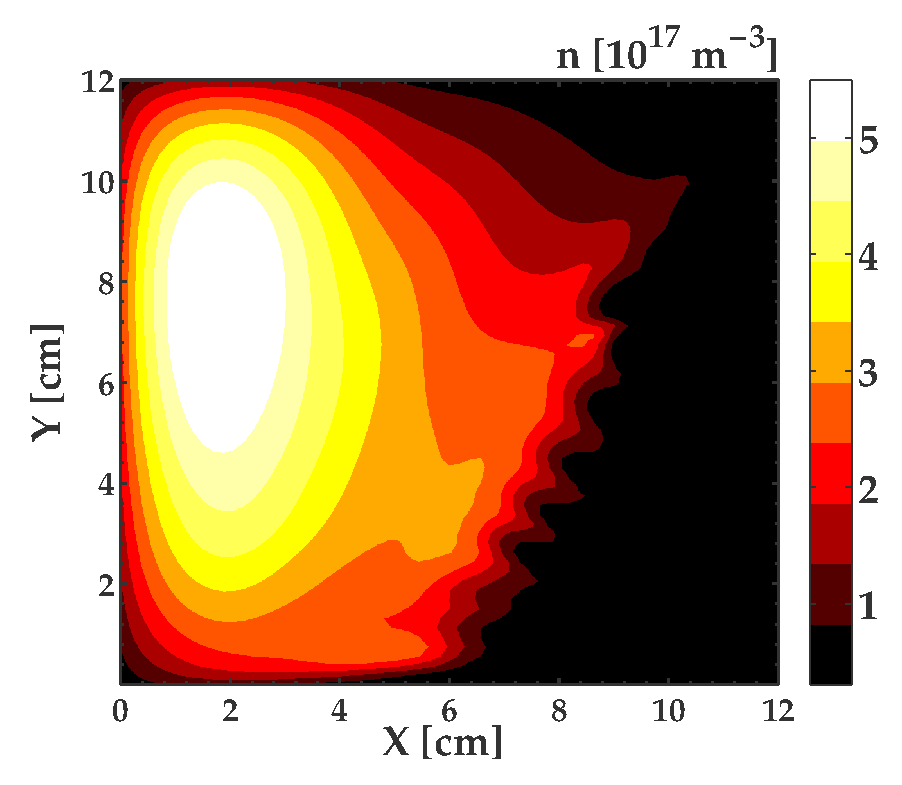
\includegraphics[height=5cm]{figures/4-PegasesCarteDensiteVarBias5.eps}
    \caption{Cartes de densité pour une pression de gaz de 10mTorr et un bias
    appliqué de 30V.}
\end{figure}
	
	
\section{Colonne de plasma magnétisée - CYBELE}

\subsection{Caractéristiques de la source}

\begin{figure}[htbp]
  \centering
    \subfigure[]{\label{4-cybelePhoto}
    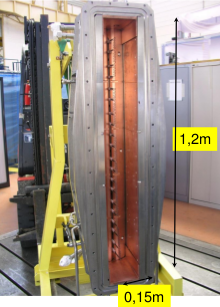
\includegraphics[height=12cm]{figures/4-cybelePhoto.png}}
    \subfigure[]{\label{4-cybeleSchema}
    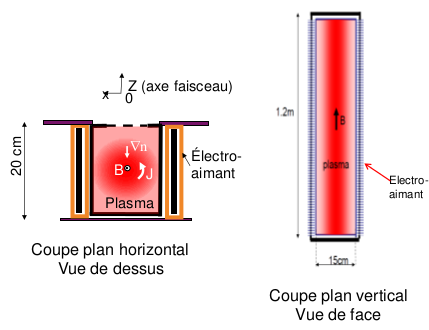
\includegraphics[height=10cm]{figures/4-cybeleSchema.png}}
    \caption{Cartes de densité\subref{4-cybelePhoto}~, de
    potentiel\subref{4-cybeleSchema}}
    \label{pandas}
\end{figure}	

a

\begin{figure}[htbp]
\centering
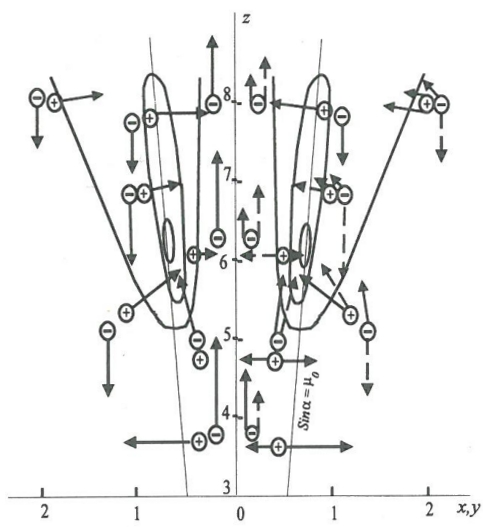
\includegraphics[width=0.8\textwidth]{figures/4-magnetizedColumn.jpg}
{\caption{Transport des ions et des électrons dans une colonne de
plasma\parencite{Rozhansky}.}
\label{4-magnetizedColumn}}
\end{figure}

\subsection{Simulation d'un plasma classique}


\begin{figure}[htbp]
\centering
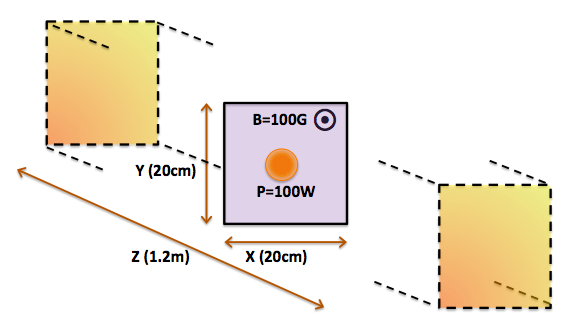
\includegraphics[width=0.8\textwidth]{figures/4-cybeleSimDomain.png}
{\caption{Le domaine de simulation est le plan perpendiculaire au champ
magnétique.}
\label{4-cybeleSimDomain}}
\end{figure}

a

\begin{figure}[htbp]
  \centering
    \subfigure[]{\label{4-CybeleCarteDensiteBase}
    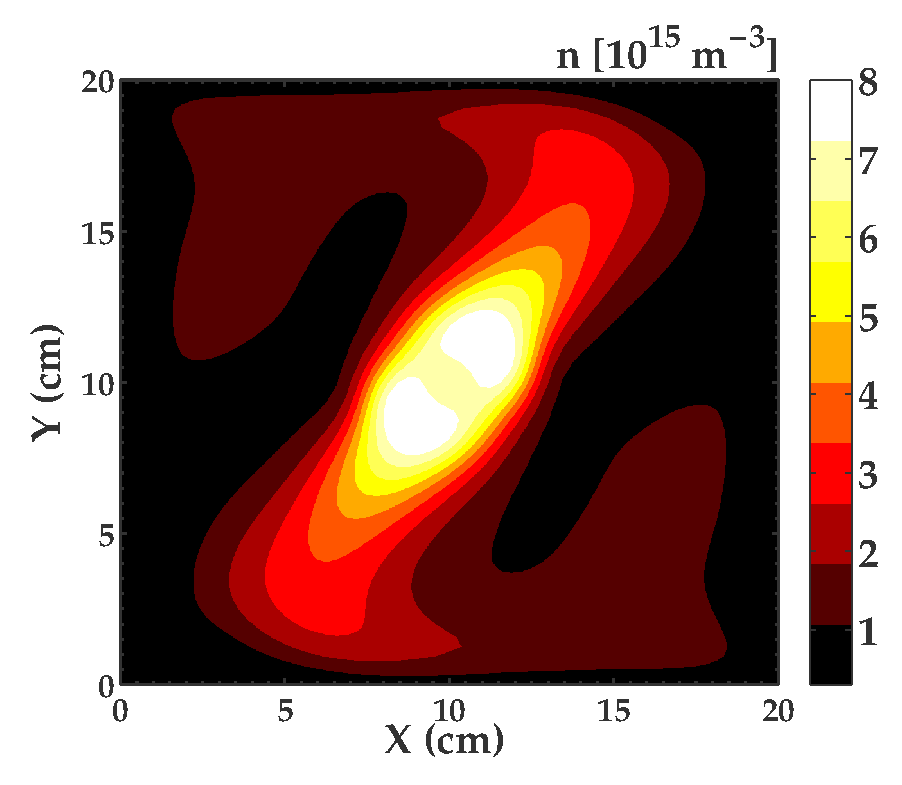
\includegraphics[height=5.5cm]{figures/4-CybeleCarteDensiteBase.eps}}
    \subfigure[]{\label{4-CybeleCartePotentielBase}
    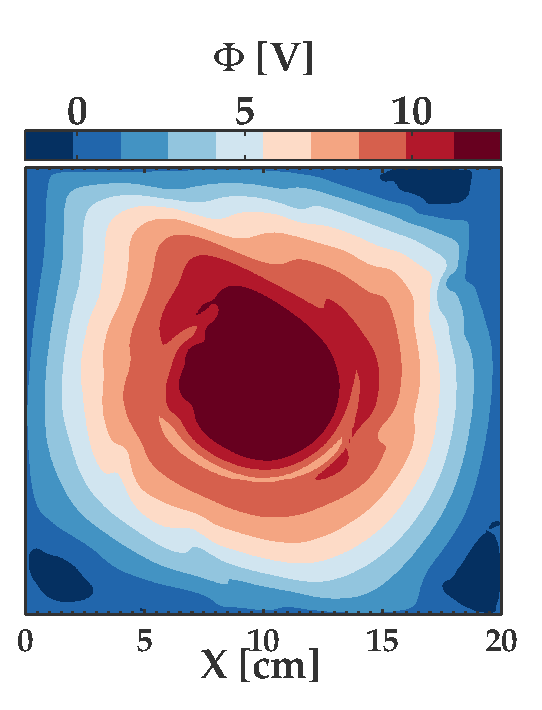
\includegraphics[height=5.5cm]{figures/4-CybeleCartePotentielBase.eps}}
    \subfigure[]{\label{4-CybeleCarteTemperatureBase}
    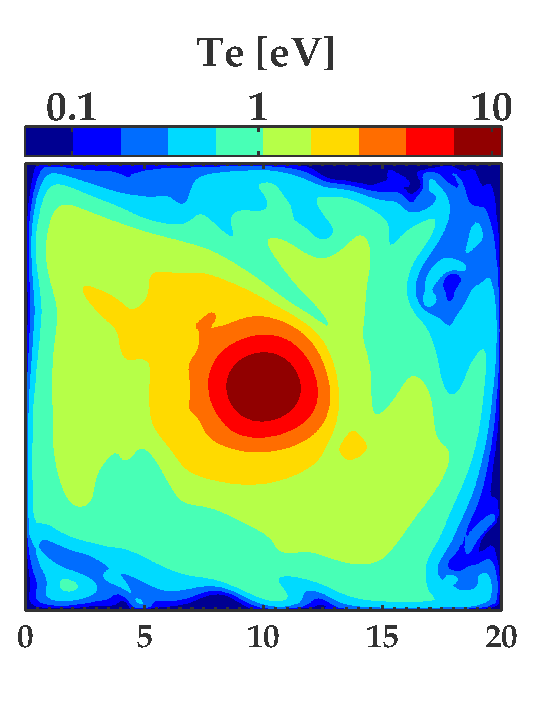
\includegraphics[height=5.5cm]{figures/4-CybeleCarteTemperatureBase.eps}}
    \caption{Cartes de densité \subref{4-CybeleCarteDensiteBase}~, de
    potentiel \subref{4-CybeleCartePotentielBase}~ et de
    température \subref{4-CybeleCarteTemperatureBase}}
    \label{pandas}
\end{figure}

a

\begin{figure}[htbp]
  \centering
    \subfigure[]{\label{4-CybeleProfilsRadial}
    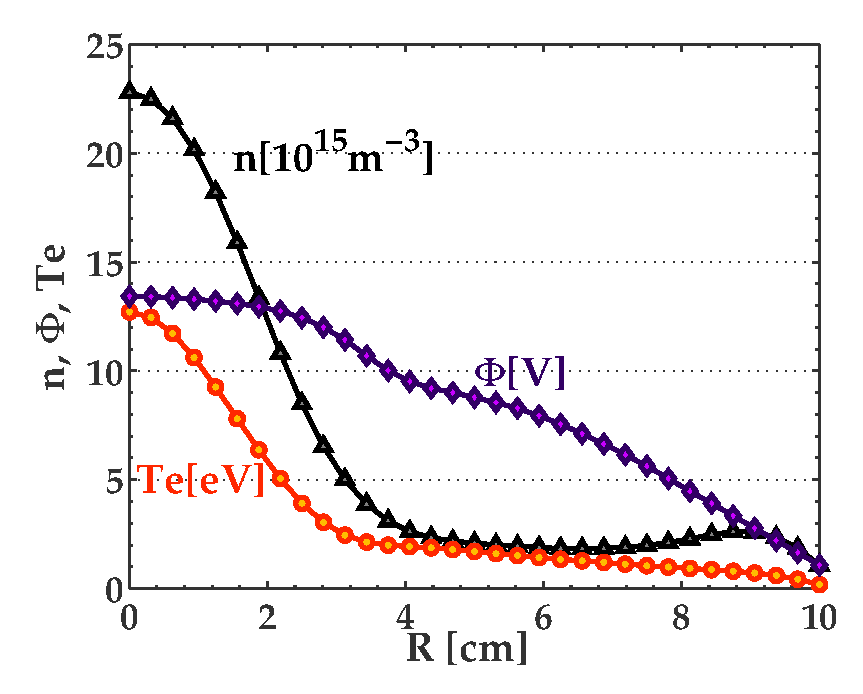
\includegraphics[height=5.2cm]{figures/4-CybeleProfileTempRadiale.eps}}
    \subfigure[]{\label{4-CybeleProfilsPol}
    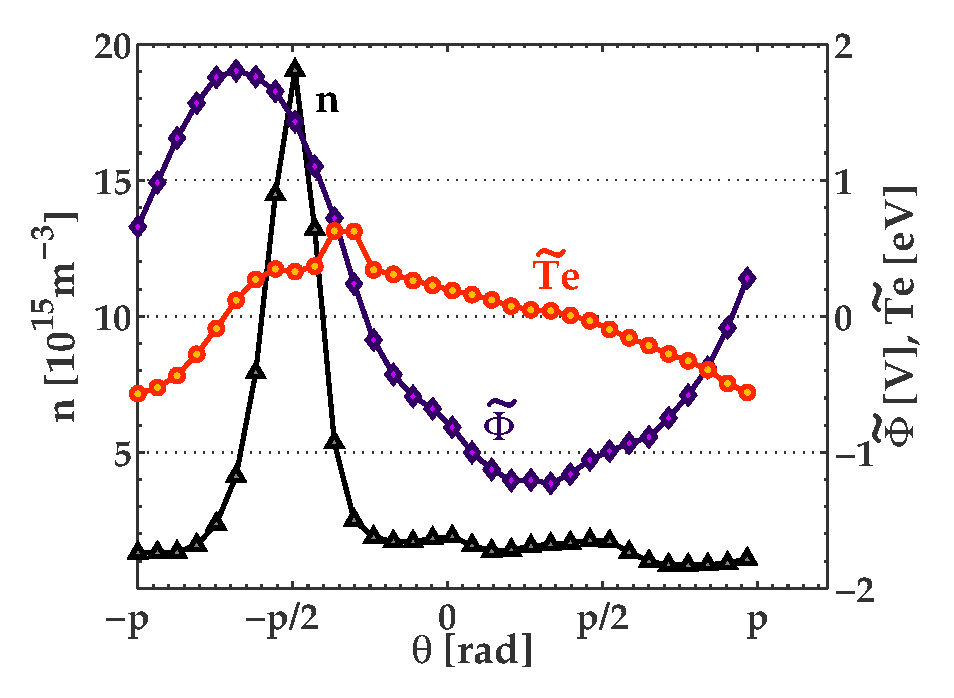
\includegraphics[height=5.2cm]{figures/4-CybeleProfileTempPol.eps}}
    \caption{Profils radiaux\subref{4-CybeleProfilsPol}~ et
    poloïdaux~\subref{4-CybeleProfilsPol} de la densité, du potentiel et de la
    température.}
    \label{4-CybeleProfils}
\end{figure}

a
\begin{figure}[htbp]
\centering
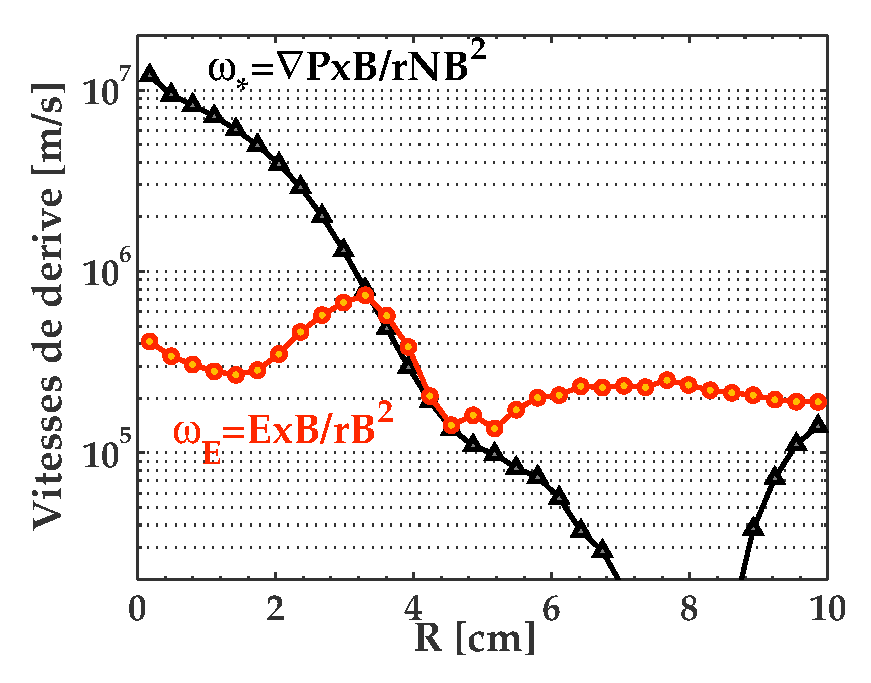
\includegraphics[width=0.5\textwidth]{figures/4-CybeleProfileVitessesDerive.eps}
{\caption{Carte de densité à 35G.}
\label{4-CybeleVitessesDerive}}
\end{figure}


\begin{figure}[htbp]
  \centering
    \subfigure[]{\label{4-CybeleCarteFluxIBase}
    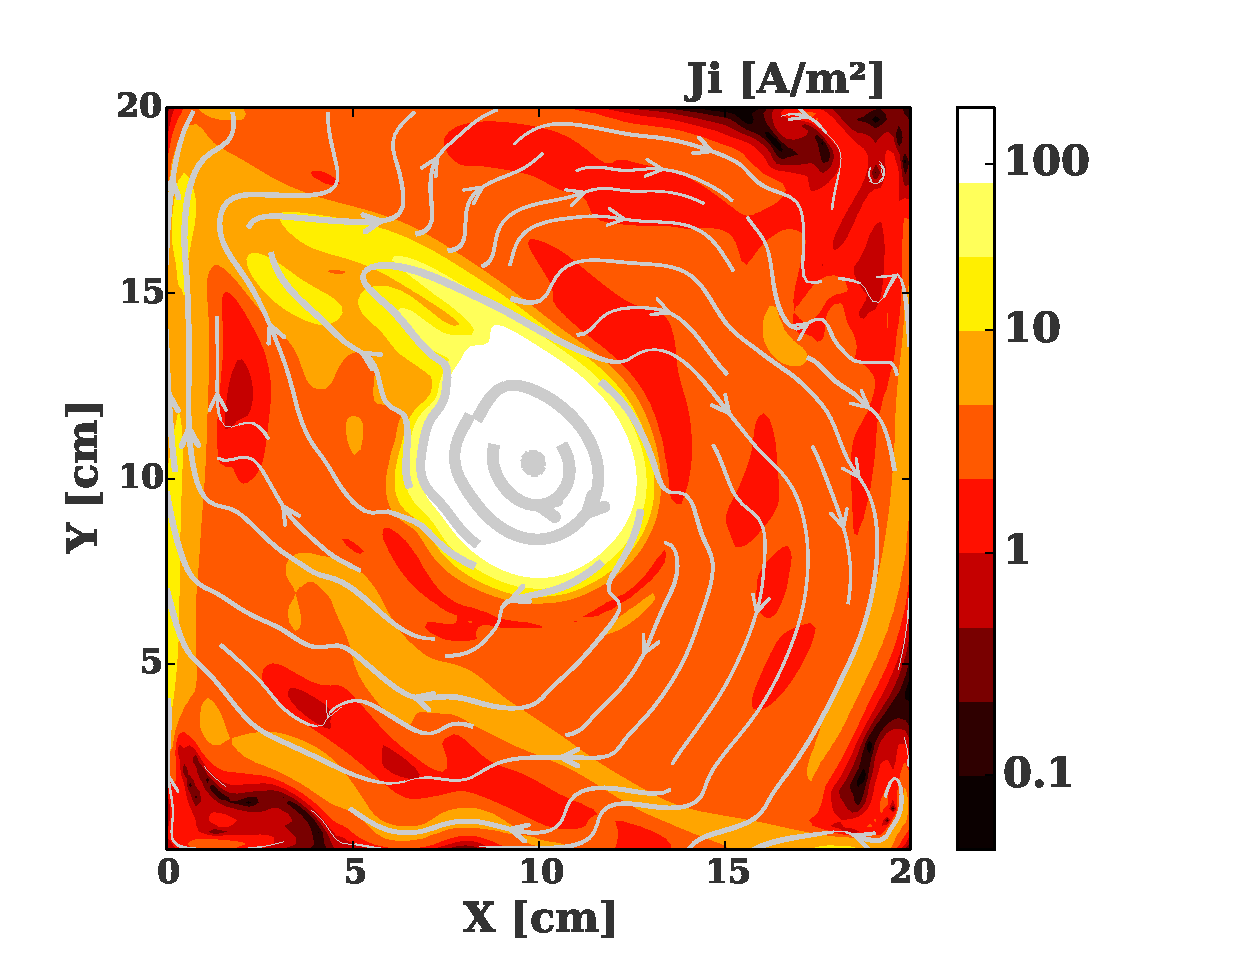
\includegraphics[height=5.5cm]{figures/4-CybeleCarteFluxIBase.eps}}
    \subfigure[]{\label{4-CybeleCarteFluxEBase}
    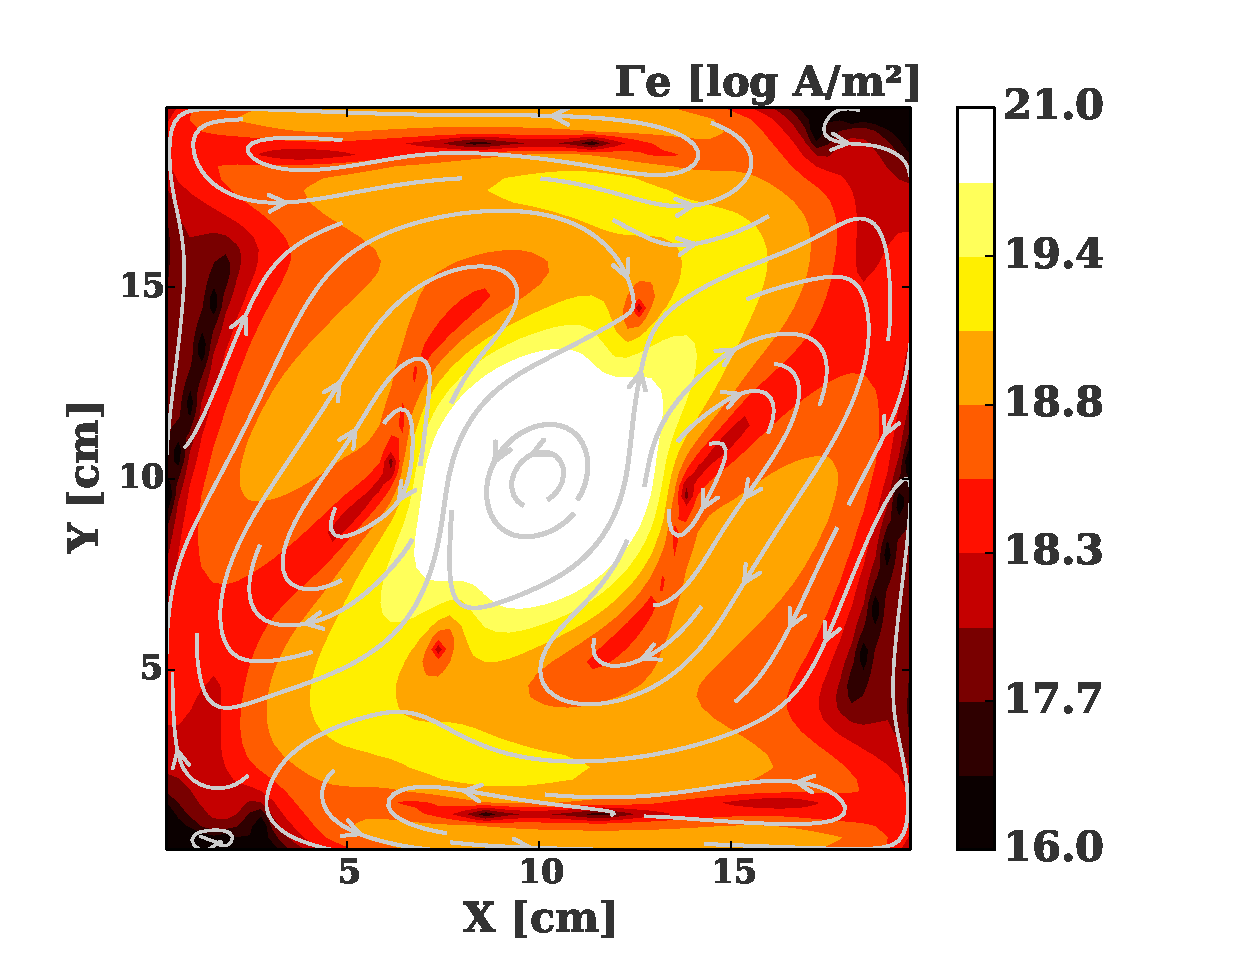
\includegraphics[height=5.5cm]{figures/4-CybeleCarteFluxEBase.eps}}
    \caption{Cartes de densité \subref{4-CybeleCarteFluxEBase}~ et de
    température \subref{4-CybeleCarteCourant}}
    \label{pandas}
\end{figure}

a

\subsection{Variation croissante du champ magnétique}

\begin{figure}[htbp]
  \centering
    \subfigure[]{\label{4-CybeleVarMag1}
    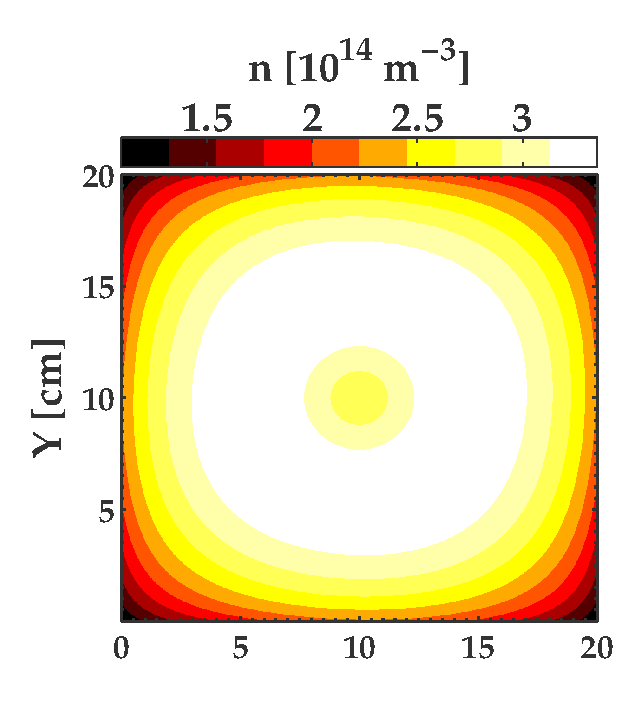
\includegraphics[height=5.5cm]{figures/4-CybeleVarMag1.eps}}
    \subfigure[]{\label{4-CybeleVarMag2}
    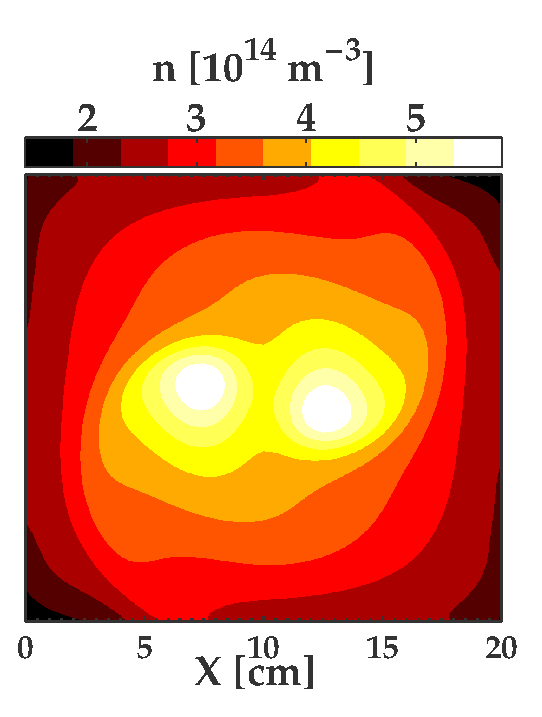
\includegraphics[height=5.5cm]{figures/4-CybeleVarMag2.eps}}
    \subfigure[]{\label{4-CybeleVarMag3}
    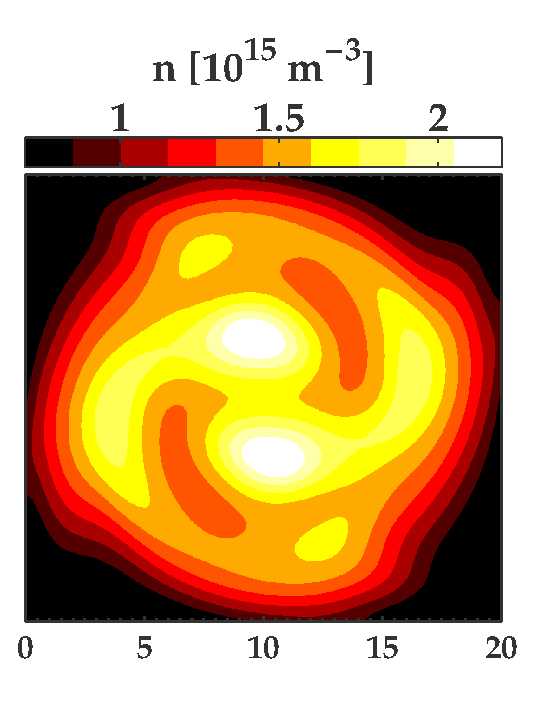
\includegraphics[height=5.5cm]{figures/4-CybeleVarMag3.eps}}
    \caption{Cartes de densité à 1G\subref{4-CybeleVarMag1}~, 4G
    \subref{4-CybeleVarMag2}~ et 15G \subref{4-CybeleVarMag3}}
    \label{pandas}
\end{figure}

a

\begin{figure}[htbp]
  \centering
    \subfigure[]{\label{4-CybeleVarMag4}
    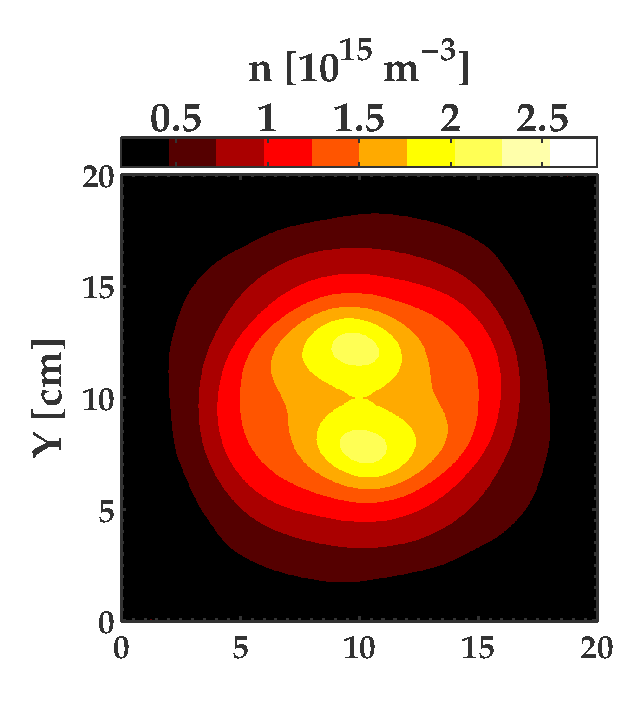
\includegraphics[height=5.5cm]{figures/4-CybeleVarMag4.eps}}
    \subfigure[]{\label{4-CybeleVarMag5}
    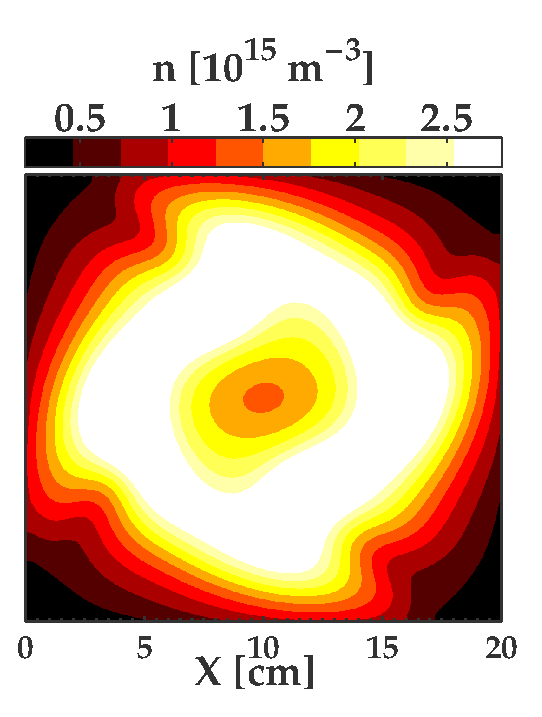
\includegraphics[height=5.5cm]{figures/4-CybeleVarMag5.eps}}
    \subfigure[]{\label{4-CybeleVarMag6}
    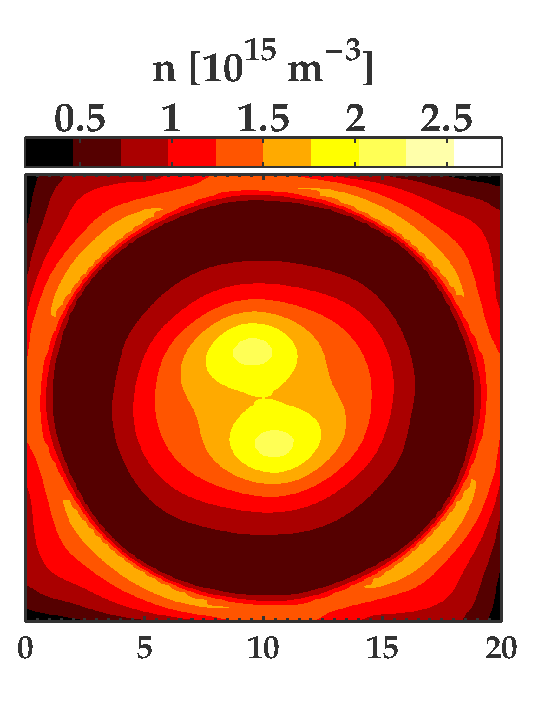
\includegraphics[height=5.5cm]{figures/4-CybeleVarMag6.eps}}
    \caption{Cartes de densité à 20G\subref{4-CybeleVarMag4}~, de
    potentiel \subref{4-CybeleVarMag5}~ et de
    température \subref{4-CybeleVarMag6}}
    \label{pandas}
\end{figure}

a

\begin{figure}[htbp]
\centering
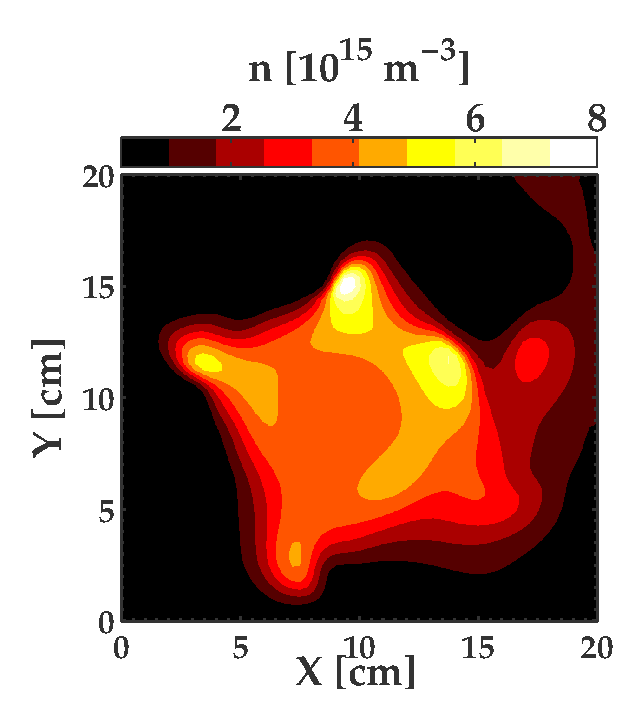
\includegraphics[width=0.5\textwidth]{figures/4-CybeleVarMag8.eps}
{\caption{Carte de densité à 35G.}
\label{4-CybeleVarMag8}}
\end{figure}

a

\begin{figure}[htbp]
  \centering
    \subfigure[]{\label{4-CybeleVarMag9}
    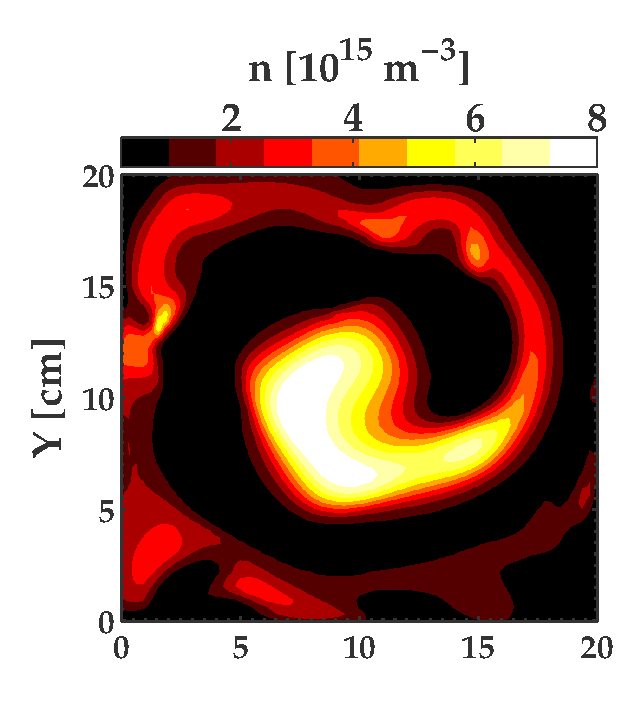
\includegraphics[height=5.5cm]{figures/4-CybeleVarMag9.eps}}
    \subfigure[]{\label{4-CybeleVarMag10}
    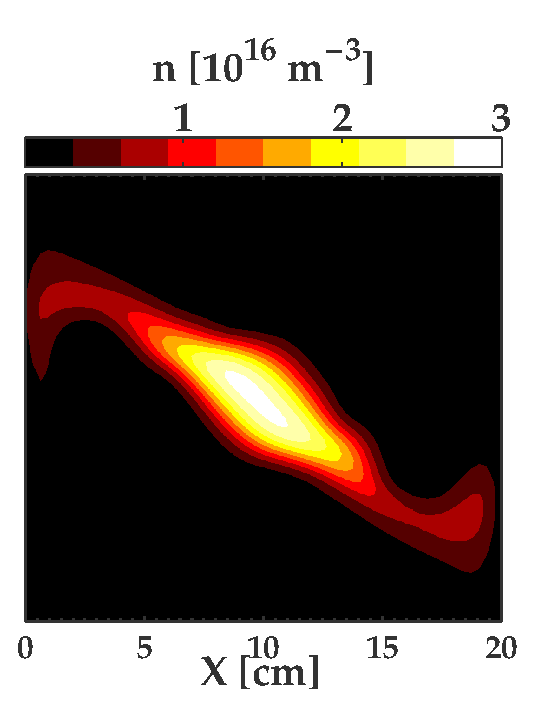
\includegraphics[height=5.5cm]{figures/4-CybeleVarMag10.eps}}
    \subfigure[]{\label{4-CybeleVarMag11}
    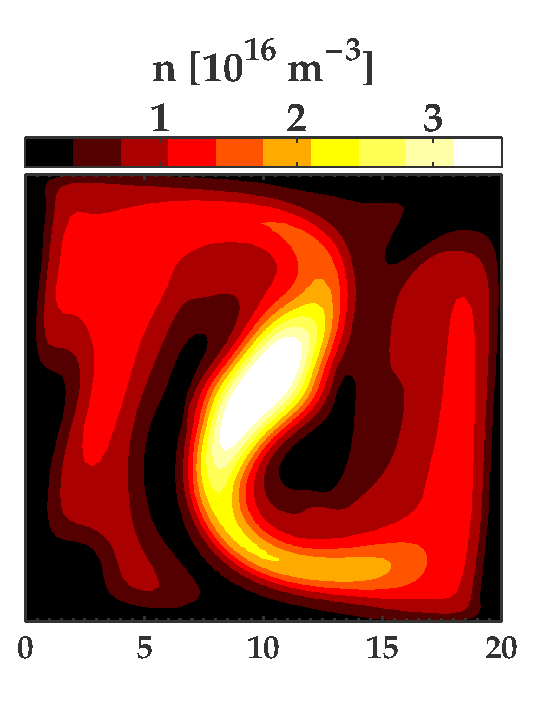
\includegraphics[height=5.5cm]{figures/4-CybeleVarMag11.eps}}
    \caption{Cartes de densité à 80G\subref{4-CybeleVarMag9}~, 130G
    \subref{4-CybeleVarMag10}~ et 170G \subref{4-CybeleVarMag11}}
    \label{pandas}
\end{figure}

a
\begin{table*}
\footnotesize\centering
\ra{1.3}
\begin{tabular}{@{}cccccccccc@{}}\toprule
B&&\multicolumn{3}{c}{Échelles} && \multicolumn{2}{c}{Champs} &&
Rotation\\
\cmidrule{3-5} \cmidrule{7-8} \cmidrule{10-10}
&& $\omega_c$ & $\rho\indice{L}$& $l_{\text{lpm}}$&& $n$ & $T_e$ && 
$\Omega_r$\\
\midrule Phase 1\\
\scriptsize 1-15 &&\scriptsize 10\textsuperscript{4} - 2 10\textsuperscript{5} &
\scriptsize0.1692 &\scriptsize 0.2945 && \scriptsize0.3670 &\scriptsize 0.7187
&& \scriptsize3.1815 \\
Phase 2\\
\scriptsize1-15 &&\scriptsize 10\textsuperscript{4} - 2 10\textsuperscript{5} &
\scriptsize0.1692 &\scriptsize 0.2945 &&\scriptsize 0.3670 &\scriptsize 0.7187
&&\scriptsize 3.1815 \\
Phase 3\\
\scriptsize1-15 &&\scriptsize 10\textsuperscript{4} - 2 10\textsuperscript{5} &
\scriptsize0.1692 &\scriptsize 0.2945 &&\scriptsize 0.3670 &\scriptsize 0.7187
&&\scriptsize 3.1815 \\

\bottomrule
\end{tabular}
\caption{Captions}
\end{table*}
	
\subsection{Rôle de la direction parallèle}
\begin{figure}[htbp]
  \centering
    \subfigure[]{\label{4-CybeleProfileDenRadialeZ}
    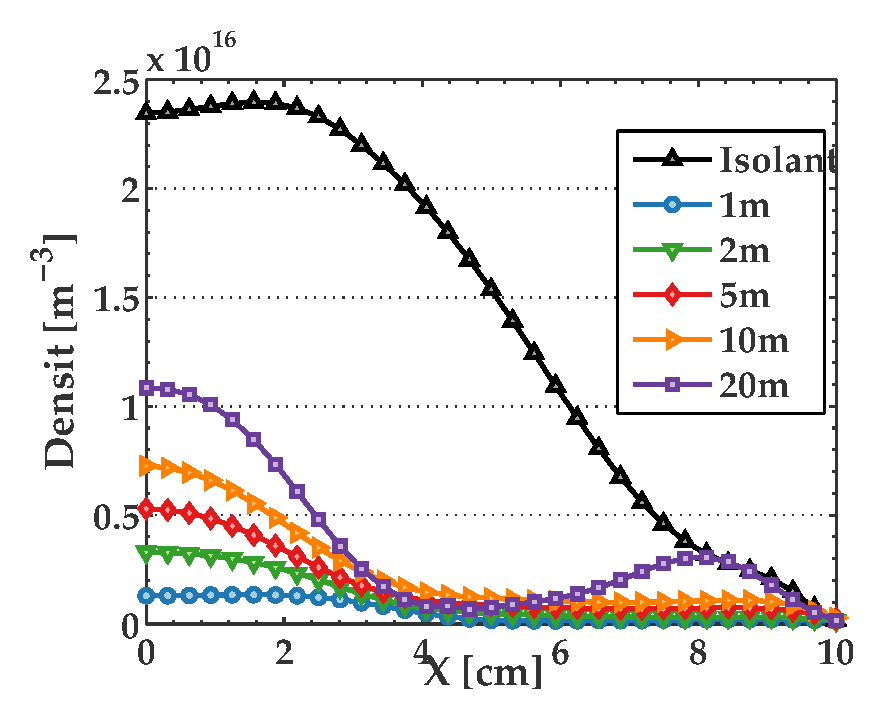
\includegraphics[height=5.25cm]{figures/4-CybeleProfileDenRadialeZ.eps}}
    \subfigure[]{\label{4-CybeleProfileTempRadialeZ}
    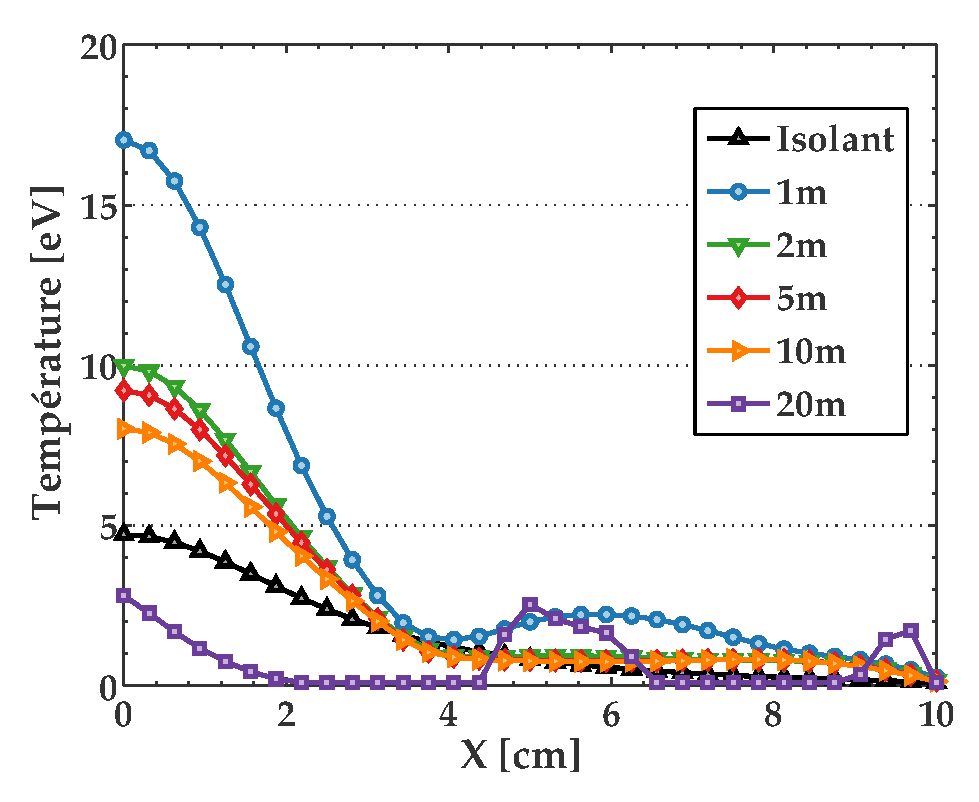
\includegraphics[height=5cm]{figures/4-CybeleProfileTempRadialeZ.eps}}
    \caption{Comparaison des profils de
    densité~\subref{4-CybeleProfileDenRadialeZ}~ et de
    température~\subref{4-CybeleProfileTempRadialeZ}~ pour différentes
    longueurs parallèles}
    \label{pandas}
\end{figure}

\begin{figure}[htbp]
\centering
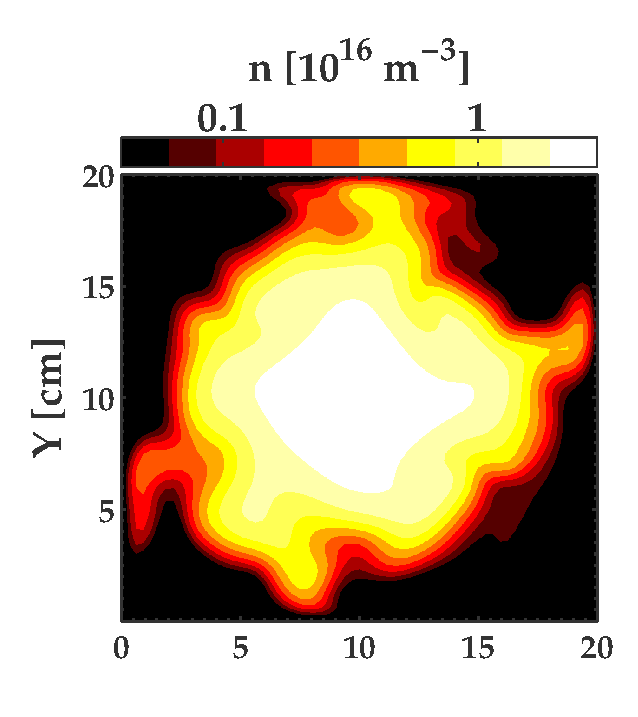
\includegraphics[width=0.5\textwidth]{figures/4-CybeleCarteDensiteIsolant.eps}
{\caption{Carte de densité pour des parois diélectriques au bout des lignes de
champ.}
\label{4-CybeleCarteDensiteIsolant}}
\end{figure}		

\section{Plasma de bord de tokamaks}
\subsection{Un cas critique pour MAGNIS}

\begin{figure}[htbp]
  \centering
    \subfigure[]{\label{4-Tokam1}
    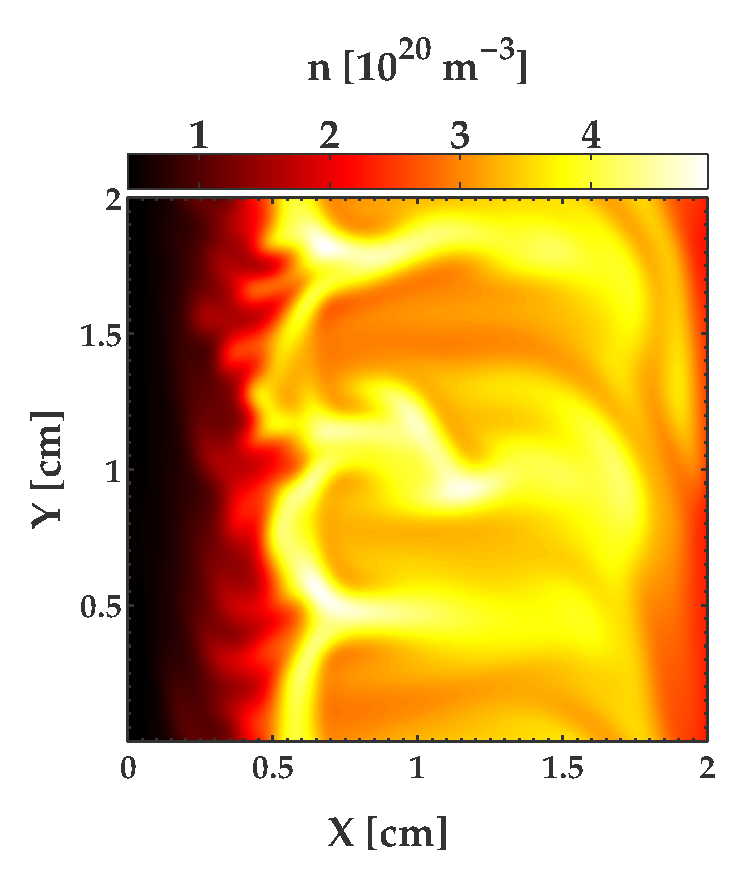
\includegraphics[height=8cm]{figures/4-Tokam1.eps}}
    \subfigure[]{\label{4-Tokam2}
    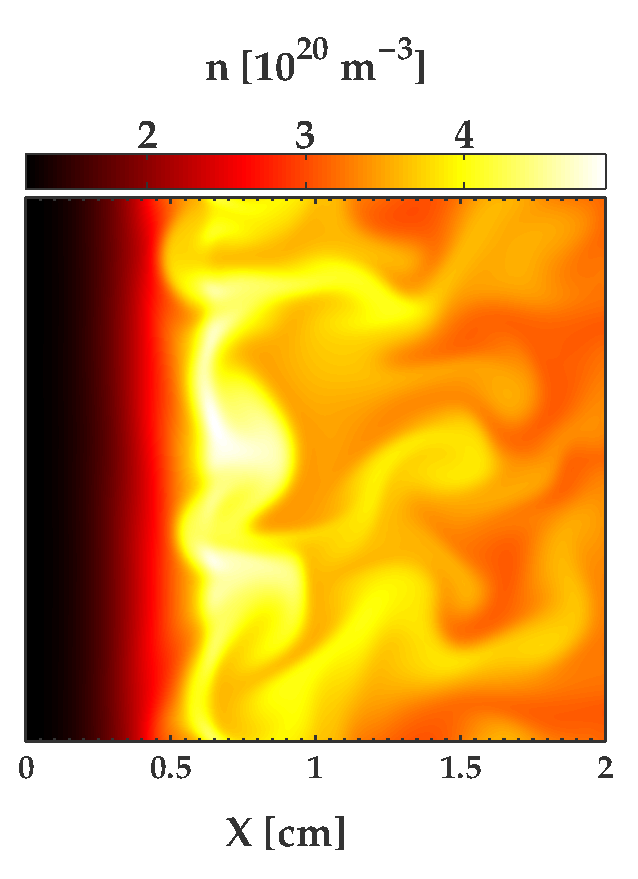
\includegraphics[height=8cm]{figures/4-Tokam2.eps}}
    \caption{Cartes de densité de la SOL simulée par
    TOKAM~\subref{4-CybeleVarMag4}~ et par MAGNIS~\subref{4-CybeleVarMag5}}
    \label{pandas}
\end{figure}
\subsection{Comparaison des profils et de la statistique}

\begin{figure}[htbp]
  \centering
    \subfigure[]{\label{4-TokamProfileDensite}
    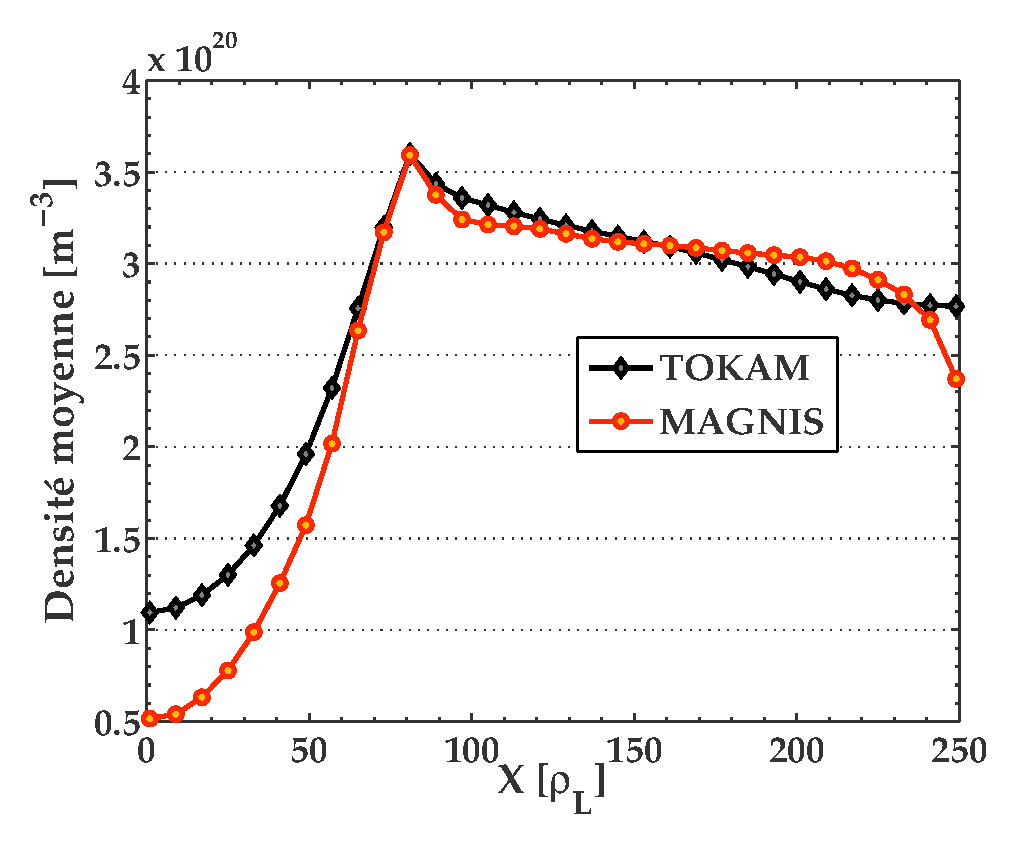
\includegraphics[height=6cm]{figures/4-TokamProfileDensite.eps}}
    \subfigure[]{\label{4-TokamProfileFluxRadial}
    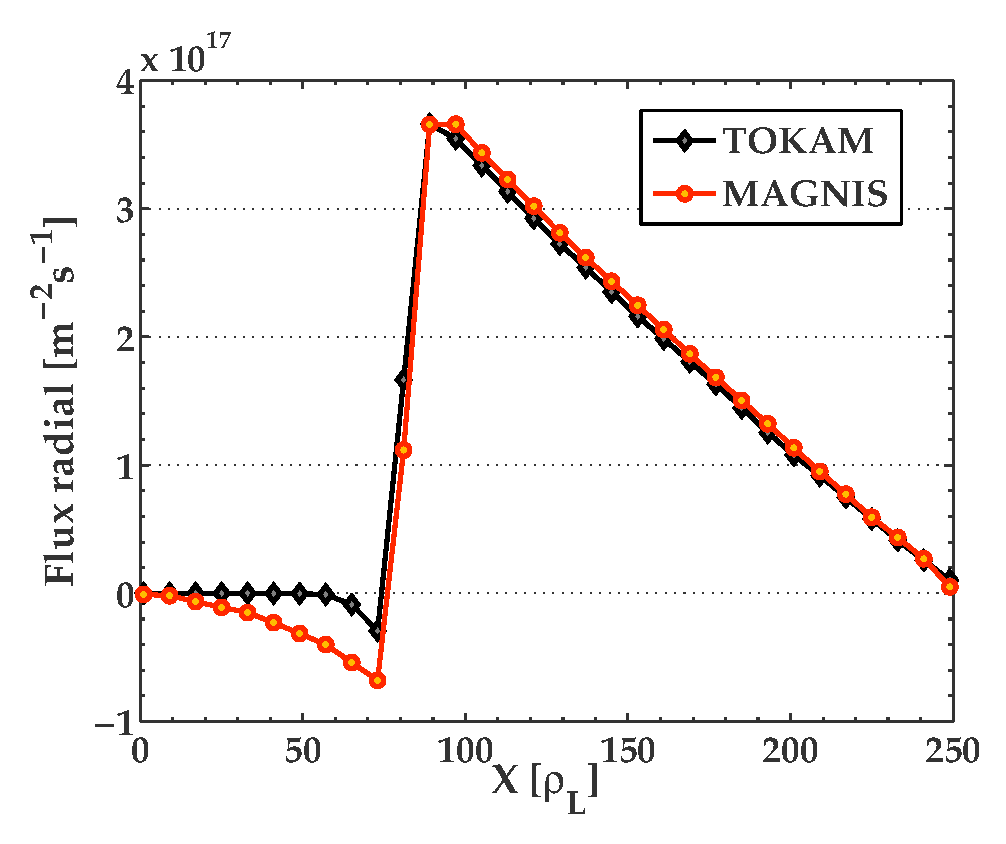
\includegraphics[height=6cm]{figures/4-TokamProfileFluxRadial.eps}}
    \caption{Comparaison des profils de
    densité~\subref{4-pegasesCompPressTempProfile}~ et de flux
    radial~\subref{4-pegasesCompPressTempProfile}~ entre TOKAM et MAGNIS}
    \label{pandas}
\end{figure}

\begin{figure}[htbp]
\centering
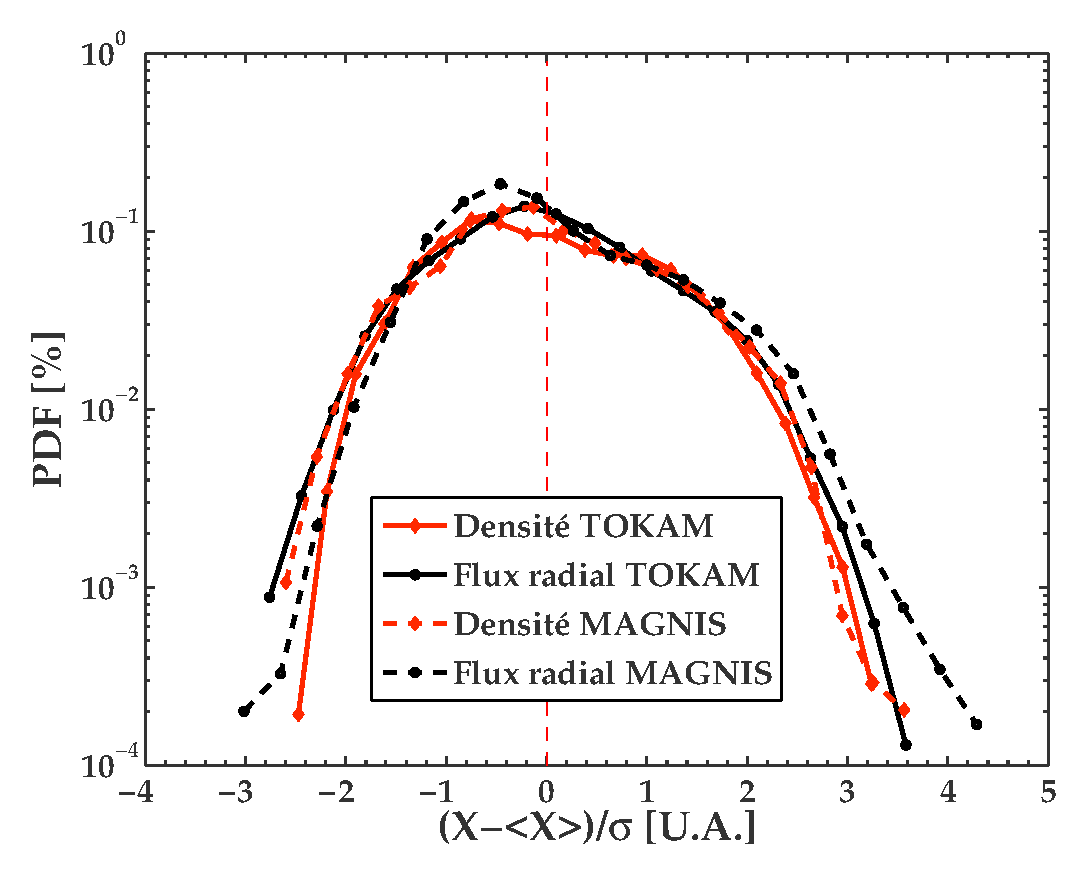
\includegraphics[width=0.5\textwidth]{figures/4-TokamPDFDensite.eps}
{\caption{Comparaisons des densités de probabilité pour la densité et
le flux radial.}
\label{4-TokamPDFDensite}}
\end{figure}

\subsection{Simulation plus complète de la SOL}
 avec une densité de neutre et la température
%\bibliographystyle{apalike}
%\bibliography{biblio}
\end{refsection}
